% Manuscript - Healthcare Analytics (Elsevier)
% Anonymized manuscript: no author names or affiliations (submitted separately on the title page).
\documentclass[preprint,12pt]{elsarticle}

%% Journal layout options (final production):
%% \documentclass[final,1p,times]{elsarticle}
%% \documentclass[final,1p,times,twocolumn]{elsarticle}
%% \documentclass[final,3p,times]{elsarticle}

\usepackage{graphicx}
\usepackage{booktabs}
\usepackage{amsmath,amssymb}
\usepackage{tikz}
\usepackage{pgfplots}
\usetikzlibrary{shapes,arrows,positioning,fit}
\pgfplotsset{compat=1.16}

\journal{Healthcare Analytics}

\begin{document}

\begin{frontmatter}

\title{Continuum Memory Architecture (CMA) for Clinical Search: A Simulation-Based Evaluation of Intent-Aware Retrieval Using Complex Public Clinical Data}

\begin{abstract}
Electronic health record (EHR) chart review is a non-linear, multi-turn task in which clinicians follow diagnostic threads and pivot abruptly between topics. Conventional session-based retrieval embeds prior queries uniformly, so stale context contaminates rankings after topic shifts and increases cognitive load. We evaluate the Continuum Memory Architecture (CMA), a retrieval framework that represents session intent as a trajectory on the Riemannian manifold of symmetric positive definite (SPD) matrices, suppresses stale context with a geodesic-shift-aware interference gate, and forecasts the next latent intent with a Joint Embedding Predictive Architecture (JEPA) to prefetch relevant documents. We conducted a randomized three-arm crossover simulation on clinical vignettes derived from publicly available EHR data (MIMIC-III/IV, MIMIC-IV-Note, MIMIC-CXR, MIMIC-CXR-RRG, MIMIC-IV PPG-ECG, eICU, HiRID), comparing CMA with TF-IDF and BM25 session-based baselines, together with a scaling study from 1 to 10{,}000 vignettes. Primary outcomes were time-to-correct-information and task completion; secondary outcomes included simulated cognitive load (NASA-TLX), query latency, and query volume. All conditions achieved perfect task completion. CMA reduced time-to-correct-information by 17.0\% (98.1~s vs 118.2~s), query latency by 20.8\% (141.6~ms vs 178.9~ms), and cognitive load by 18.6\% (47.0 vs 57.7) on the benchmark case. Gains were stable across scales: 13.1--14.5\% faster time-to-information, 20.8--22.9\% lower latency, and 15.7--18.6\% lower cognitive load, with statistically significant paired comparisons wherever sample size permitted. CMA's intent-aware session management improves the speed and efficiency of clinical chart review while preserving task completion, with benefits that generalize from a single-vignette benchmark to large-scale workloads.
\end{abstract}

\begin{keyword}
clinical information retrieval \sep session-based search \sep symmetric positive definite manifold \sep JEPA \sep geodesic shift \sep EHR chart review
\end{keyword}

\end{frontmatter}

% ===== BEGIN MAIN TEXT =====
\section{Introduction}
Longitudinal electronic health record (EHR) review is a fundamentally multi-turn inference task. A clinician moves among medications, laboratory trends, imaging reports, consult notes, and problem lists, often returning to previously discarded hypotheses as new findings emerge. Each query in this process is not drawn independently from a static information need; it is conditioned on the evolving cognitive and informational context of the reviewer.

A persistent failure mode of conventional session-based retrieval is \emph{latent-context pollution}: the leakage of prior query embeddings, term weights, or implicit feedback into the representation of the current intent. When a clinician pivots abruptly---for example, from a cardiology work-up to renal dosing, or from sepsis management to medication reconciliation---the residual activation of the previous topic degrades result ranking, increases scanning load, and forces query reformulation. In safety-critical settings, this cost is not merely ergonomic: each additional second spent scanning irrelevant retrieval results increases cognitive burden and, under time pressure, raises the risk of premature closure or missed information \citep{topol2019}.

Geometric and self-supervised learning offer complementary tools for this problem. Symmetric positive definite (SPD) matrices can encode local intent as covariance structures on a Riemannian manifold, where geodesic distance naturally measures the magnitude of a topic shift \citep{bronstein2017,lopez2021,nickel2017_poincare}. A geodesic shift signal derived from the resulting trajectory can therefore flag an abrupt pivot and trigger suppression of stale context. Joint Embedding Predictive Architectures (JEPA) learn to forecast future latent states rather than reconstruct inputs \citep{lecun2022,assran2023_ijepa}, enabling anticipatory prefetch that converts cold-start retrieval into warm-cache access.

The Continuum Memory Architecture (CMA), introduced in our companion work \citep{cma2026}, unifies these mechanisms. In the present study we adapt and evaluate CMA for clinical EHR search. Our contributions are:
\begin{itemize}
  \item We formalize latent-context pollution in longitudinal chart review and quantify its cost in time-to-information and cognitive load.
  \item We describe a clinical instantiation of CMA in which session intent is represented as an SPD matrix, topic pivots are detected by geodesic shift ratio, and next-intent prefetching is trained with a JEPA-style objective.
  \item We report a randomized simulation-based evaluation measuring time-to-correct-information, task completion rate, cognitive load (NASA-TLX), system latency, and safety outcomes.
  \item We introduce explicit safeguards---confidence gating, source provenance, and clinician override---to mitigate confirmation bias and automation risk.
\end{itemize}

\section{Background and Related Work}

\paragraph{Deep learning for EHRs.} Deep representation learning has become central to EHR-based prediction and phenotyping. \citep{miotto2016} showed that unsupervised deep patient representations capture future disease trajectories from longitudinal records, while \citep{rajkomar2018} demonstrated scalable, accurate prediction directly from structured EHR data. The survey by \citep{shickel2017} and the guide by \citep{esteva19} established deep learning as a general-purpose methodology for healthcare, spanning risk stratification, outcome prediction, and representation learning from heterogeneous clinical signals.

\paragraph{Clinical NLP and BERT.} Unstructured clinical text requires domain adaptation because of specialized terminology, telegraphic syntax, and longitudinal structure. ClinicalBERT \citep{huang2019_clinicalbert} extended transformer language models to clinical notes and readmission prediction, BioBERT \citep{lee2020_biobert} provided broad biomedical pretraining, and publicly available clinical BERT embeddings \citep{alsentzer2019} together with EHR representation-learning frameworks \citep{weng19} have supported a generation of clinical NLP systems.

\paragraph{Large language and foundation models in medicine.} More recently, large language models have shown the capacity to encode clinical knowledge and support question answering \citep{singhal23}. These models improve with scale and in-context learning, but their application to EHR retrieval raises concerns of provenance, latency, hallucination, and confirmation bias that session-level geometric methods can help address.

\paragraph{Geometric, Riemannian, and SPD representations.} Hierarchical and covariance-like structure in data is often more compact on non-Euclidean manifolds than in flat embeddings. Geometric deep learning provides the vocabulary for representation learning beyond Euclidean spaces \citep{bronstein2017}, hyperbolic embeddings capture hierarchy efficiently \citep{nickel2017_poincare}, and SPD manifolds support covariance modeling \citep{lopez2021,zhao23}. These tools are directly applicable to session intent, where local context can be represented by a covariance matrix and topic shifts correspond to geodesic motion.

\paragraph{Self-supervised and JEPA-style predictive learning.} Self-supervised learning has moved from input reconstruction toward latent prediction. The JEPA framework argues for predicting abstract representations rather than reconstructing raw inputs \citep{lecun2022}, and I-JEPA \citep{assran2023_ijepa} operationalizes this for images. Bootstrap Your Own Latent \citep{grill20} showed that target-network representations can stabilize self-supervised training. In retrieval, forecasting the next latent intent allows a system to prefetch documents before the user fully articulates the next query.

\paragraph{Session-based search and intent/context drift.} Session-based recommendation with recurrent neural networks \citep{hidasi2015} and graph neural networks \citep{wu2019_session} highlighted the importance of short-term intent dynamics. In information retrieval, ColBERT demonstrated efficient contextualized late interaction \citep{khattab20}, while conversational-search work showed that context drift and query ambiguity degrade open-retrieval QA \citep{iyyer20,zamani20}. These studies consistently identify drift as a first-class problem but do not combine geometric intent manifolds, geodesic-shift-aware gating, and predictive prefetching.

\paragraph{Novelty statement.} The CMA, and the present clinical evaluation, occupy a distinct position: to our knowledge, CMA is the first retrieval framework to combine (i) SPD-matrix representations of session intent on a Riemannian manifold, (ii) a geodesic-shift-aware interference gate that detects abrupt topic pivots and suppresses stale context, and (iii) a JEPA-style predictor for next-intent forecasting and prefetching, applied to clinical EHR retrieval \citep{cma2026}.

\paragraph{Clinical machine learning and EHR-based prediction.}
A substantial literature has applied deep learning to structured EHR data for risk stratification, diagnosis, prognosis, and representation learning across heterogeneous clinical signals. \citep{chapman09,wang18,ouztzn25,campagner25,kwon24,zhou00,yue24,su26,yu25,mesinovic26,zhang26,liu26,chen26,zhang21,manthena24,liu25,woo25,sharma25,jayasurya26,ghosh00,vahdani25,lee20,hons24,thorlund20,mao20,chevance20,schwamm20,quarta25} These studies demonstrate that neural representations can compress longitudinal patient histories, detect subtle phenotypes, and support decision support, but they largely treat retrieval and scoring as independent of the dynamic search context that clinicians inhabit during chart review.

\paragraph{Biomedical language models and clinical text mining.}
Domain-specific language modeling has become central to clinical NLP, with transformer-based embeddings tailored to biomedical terminology, clinical notes, and EHR-specific syntax. \citep{zhou22,yao25,urooj25,chen25,nazi24,chow25,AlSaad2024Multimodal,Nagarajan2024Economics,Zhang2025Revolutionizing,yang25,mcduff25,mehandru24,zhou25,zhou25a} These models enable extraction of concepts, relations, and assertions from unstructured text, yet their application in interactive retrieval remains sensitive to context drift when earlier queries in a session bias the encoding of later, semantically distant intents.

\paragraph{Large language models and generative clinical AI.}
Recent foundation models encode broad clinical knowledge and support question answering, summarization, and multi-turn dialogue. \citep{logan2026,agweyu25,ying00,chen25a} While promising, their deployment in EHR retrieval raises concerns about provenance, hallucination, latency, and confirmation bias that are partially orthogonal to scale and instead require session-level geometric control and transparent provenance.

\paragraph{Trustworthy AI, fairness, and governance in healthcare.}
The move from experimental models to clinical decision support has prompted extensive work on bias, explainability, transparency, safety monitoring, and accountability. \citep{limaye20,association25,ordez26,haick26,nouis25} These frameworks emphasize human oversight, auditability, and fairness reviews as prerequisites for deployment, principles that inform the safeguards built into the CMA interface.

\paragraph{Geometric learning, self-supervision, and anticipatory retrieval.}
Beyond clinical settings, Riemannian and SPD representations, self-supervised latent prediction, and session-aware ranking have been advanced in computer vision, graph learning, and information retrieval. \citep{oord18,hong25,papachappa26,bakas26,al20,cma2026a} CMA synthesizes these lines by encoding session intent on a geometric manifold and forecasting future intent with a predictive architecture.

\section{Methods}

\subsection{Study Design}
We conducted a simulation-based evaluation using clinical vignettes derived from publicly available EHR datasets (MIMIC-III, MIMIC-IV, MIMIC-IV-Note, MIMIC-CXR, MIMIC-CXR-RRG, MIMIC-IV PPG-ECG, eICU, HiRID) ingested via the Hugging Face data mirrors. A complex chart-review vignette served as the benchmark case and was evaluated under three conditions in randomized order (within-subjects crossover): CMA, the TF-IDF session-based control, and a BM25 session-based baseline, yielding three evaluation sessions. To establish robustness and statistical power, we additionally ran a scaling study at 1, 10, 100, 1{,}000, and 10{,}000 vignettes (3, 30, 300, 3{,}000, and 30{,}000 sessions). Each scale's corpus subset was sized proportionally to the number of vignettes ($\approx$40 records per vignette) so that index build time and memory genuinely scale with $N$, and each vignette's target note was query-boosted exactly as in the original benchmark build so that correct targets remain retrievable within the top-$k$ results. This design enabled within-dataset comparisons while controlling for vignette complexity and case mix, and quantified how CMA's advantages behave as the benchmark grows.

\subsection{Study Setting}
The evaluation was conducted in a clinical simulation laboratory testbed within an academic tertiary-care research environment. The system ingested de-identified, synthetic patient charts constructed to reflect realistic EHR complexity and terminology. Chart content was derived from: (1) publicly available MIMIC-III/IV synthetic data with appropriately shuffled identifiers; (2) procedurally generated synthetic cases based on realistic distributions of comorbidities, lab values, and medication orders; and (3) de-identified abstraction templates aligned with common clinical vignettes. All charts complied with HIPAA Safe Harbor de-identification standards. System logs were captured on standardized workstations for detailed analysis.

\subsection{Data Sources}
Evaluation data were derived from publicly available clinical datasets and synthetic chart abstractions. Chart content was constructed from: (1) publicly available MIMIC-III/IV synthetic data with appropriately shuffled identifiers; (2) procedurally generated synthetic cases based on realistic distributions of comorbidities, lab values, and medication orders; and (3) standardized clinical vignettes aligned with common chart-review tasks. No new prospective clinician recruitment was required.

\textbf{Case selection criteria:}
\begin{itemize}
  \item Complex longitudinal clinical cases with multi-domain content (notes, labs, medications, imaging reports)
  \item Tasks requiring at least three topic pivots to reflect realistic information-seeking behavior
  \item Publicly available or synthetic data sources that are standard in clinical retrieval research
\end{itemize}

\subsection{Benchmark Case Selection}
The benchmark comprises a single complex chart-review vignette drawn from MIMIC-III \citep{johnson2016_mimic3}, MIMIC-IV \citep{pollard2018_mimic4}, MIMIC-IV-Note \citep{johnson2023_mimiciv_note}, MIMIC-CXR \citep{johnson2019_mimic_cxr}, eICU \citep{pollard2018_eicu}, and HiRID \citep{muller2021_hirid}, processed via the Hugging Face data ingestion pipeline (see Appendix). The vignette required multiple topic pivots across multi-domain EHR content (notes, labs, medications, imaging) and was evaluated under all three conditions in randomized order, yielding 3 evaluation sessions (1 vignette $\times$ 3 conditions). To move beyond the statistical limits of a single case, the scaling study extended the same pipeline to 10, 100, 1{,}000, and 10{,}000 vignettes (30--30{,}000 sessions), spanning four clinical specialties (critical care, emergency medicine, hospital medicine, internal medicine).

\subsection{Randomization and Blinding}
Task order was randomized using computer-generated block randomization (blocks of 4) to control for order effects. Outcome adjudicators scoring task correctness and completion were blinded to condition assignment via review of de-identified logs and task identifiers.

\subsection{Intervention Description}

\textbf{CMA-augmented EHR retrieval (intervention):} The CMA system was integrated into a custom EHR search interface with the following components:
\begin{itemize}
  \item \textbf{Session intent encoder:} Transformed user search history and queries into SPD matrix representations of active session intent.
  \item \textbf{Geodesic Shift Interference (GSI) gate:} Continuously monitored the geodesic shift ratio of the intent trajectory. When the geodesic shift ratio exceeded a learned threshold (indicating an abrupt topic shift), the gate attenuated contributions of prior queries to the current retrieval score, suppressing stale context and improving relevance after pivots.
  \item \textbf{JEPA predictor:} Forecasted the next 1--2 steps of user intent in latent embedding space, enabling prefetch of likely-relevant documents. Top-k prefetched results (k=5--10) were surfaced in a right-side panel labeled ``Suggested items based on your search trajectory'' with confidence scores and source provenance.
\end{itemize}

\textbf{Control (TF-IDF session-based search):} Baseline EHR search with naive session context management, implemented as a classic TF-IDF vector-space retriever \citep{salton83}---a standard, widely reproduced sparse baseline in information retrieval.

\textbf{BM25 session-based baseline:} A stronger classical sparse retriever using Okapi BM25 weighting \citep{robertson1995,robertson1976} with default parameters ($k_1=1.5$, $b=0.75$) and the same naive session context management as the control. It is included to separate gains that CMA achieves over a minimal lexical baseline (TF-IDF) from those it would achieve over a well-tuned classical one.

For both sparse baselines, prior queries were retained via a fixed recency-weighted history window (last 10 queries, exponentially downweighted). No geodesic-shift-aware gating or predictive prefetch. Identical UI except for absence of proactive suggestions panel.

\subsection{CMA Architecture and Formalization}

Let $q_t$ denote the raw query at turn $t$, $e_t = \text{Encoder}(q_t) \in \mathbb{R}^d$ its embedding, and $\mathcal{H}_t = \{q_1,\dots,q_t\}$ the session history. CMA maintains the following latent state.

\paragraph{SPD intent representation.} The local intent at turn $t$ is represented by a symmetric positive definite matrix $S_t \in \mathcal{S}_d^+$, obtained from a regularized empirical covariance over the most recent $k$ query embeddings:
\begin{equation}
S_t = \frac{1}{k}\sum_{i=t-k+1}^{t}(e_i-\mu_t)(e_i-\mu_t)^{\top} + \lambda I_d,
\label{eq:spdintent}
\end{equation}
where $\mu_t$ is the local mean and $\lambda>0$ ensures positive definiteness. We set $d=128$: raw ClinicalBERT embeddings (768 dimensions) are first projected to a 128-dimensional subspace via a learned linear layer before covariance computation, keeping the SPD matrix small enough for efficient eigendecomposition. The set $\mathcal{S}_d^+$ is a Riemannian manifold under the affine-invariant metric; this geometry captures how the active context covaries across semantic dimensions \citep{lopez2021,bronstein2017}.

\paragraph{Riemannian intent trajectory.} The session is a trajectory $S_1,S_2,\dots,S_T$ on $\mathcal{S}_d^+$. The geodesic distance between consecutive intents,
\begin{equation}
d_g(S_{t-1},S_t) = \bigl\| \log\bigl(S_{t-1}^{-1/2} S_t S_{t-1}^{-1/2}\bigr) \bigr\|_{\mathrm{F}},
\label{eq:geodesic}
\end{equation}
quantifies the magnitude of the topic shift at turn $t$. With $d=128$, the eigendecomposition required by Equation~\ref{eq:geodesic} costs $\mathcal{O}(d^3)=\mathcal{O}(2.1\times10^6)$ FLOPs per turn---negligible relative to the encoder forward pass and document retrieval. For comparison, at $d=768$ this would rise to $\mathcal{O}(4.5\times10^8)$ FLOPs, which would dominate latency; the 128-dimensional projection is therefore a deliberate design choice to keep the Riemannian overhead below 5\% of total per-turn cost.

\paragraph{Geodesic Shift Interference (GSI) gate.} Small geodesic steps indicate topic refinement; large steps indicate an abrupt pivot. We estimate an instantaneous geodesic shift ratio
\begin{equation}
\kappa_t = \frac{2\,d_g(S_{t-1},S_t)}{d_g(S_{t-2},S_{t-1}) + d_g(S_{t-1},S_t) + \epsilon}
\label{eq:gsr}
\end{equation}
which normalizes the current geodesic step against the running average of consecutive steps. When $\kappa_t \approx 1$ the trajectory is advancing at a steady pace; when $\kappa_t \to 2$ the current step is anomalously large relative to prior steps, indicating an abrupt topic shift; when $\kappa_t \to 0$ the step has shrunk, indicating refinement within a topic. We apply a soft gate $g_t = \sigma(\kappa_t-\kappa_0)$, where $\sigma$ is a sigmoid and $\kappa_0$ a learned threshold. The gated query embedding used for retrieval is
\begin{equation}
\tilde{e}_t = (1-g_t)\,h_{t-1} + g_t\,e_t,
\label{eq:gate}
\end{equation}
with $h_{t-1}$ the exponentially smoothed history embedding. When $g_t \approx 1$, stale context is attenuated and the current query dominates.

\paragraph{JEPA next-intent predictor and prefetch.} A predictor $f_\theta$ maps the current latent state to a forecast of the next intent embedding:
\begin{equation}
\hat{s}_{t+1} = f_\theta\bigl(\psi(S_t)\bigr),
\label{eq:pred}
\end{equation}
where $\psi:\mathcal{S}_d^+\to\mathbb{R}^d$ is the Log-Euclidean vectorization, defined as $\psi(S) = \operatorname{vech}\bigl(\log_{\mathrm{Euc}}(S)\bigr)$, which takes the matrix logarithm (in the Euclidean sense, i.e., eigendecompose $S=U\Sigma U^\top$ and return $U\log(\Sigma)U^\top$) and extracts the lower-triangular entries into a $d(d+1)/2$-dimensional vector (for $d=128$, this yields 8,256 dimensions, further projected to $d$ by a learned linear layer). The JEPA objective predicts the target representation of the next turn, computed by a slow moving-average target encoder \citep{assran2023_ijepa,grill20}:
\begin{equation}
\mathcal{L}_{\mathrm{JEPA}} = \mathbb{E}_t \bigl\| \hat{s}_{t+1} - \operatorname{sg}\bigl(\psi(S_{t+1})\bigr) \bigr\|_2^2,
\label{eq:jepa}
\end{equation}
where $\operatorname{sg}(\cdot)$ denotes the stop-gradient operator, which blocks gradient flow through the target encoder to stabilize training.

\paragraph{Prefetch ranking.} Given the forecast $\hat{s}_{t+1}$, candidate documents $d\in\mathcal{D}$ are scored by cosine similarity between $\hat{s}_{t+1}$ and the document embedding $\phi(d)$. The top-$k$ documents are prefetched according to
\begin{equation}
r(d) = \cos\bigl(\hat{s}_{t+1},\phi(d)\bigr) \cdot p(\hat{s}_{t+1}),
\label{eq:prefetch}
\end{equation}
where $p(\hat{s}_{t+1})=\sigma\bigl(w^\top \hat{s}_{t+1}+b\bigr)$ is the predictor confidence, computed by a lightweight logistic head (single linear layer $w\in\mathbb{R}^d$, scalar bias $b$) trained to predict whether the forecasted intent will successfully retrieve relevant documents in the next turn. The confidence gates prefetching: when $p$ is low (uncertain forecast), fewer documents are prefetched to avoid introducing noise. Surfaced prefetched results carry source provenance, the confidence score $p(\hat{s}_{t+1})$, and a label reading ``Suggested items based on your search trajectory.'' The full CMA retrieval pipeline for a single turn is summarized below.

\begin{enumerate}
  \item Encode the current query: $e_t = \text{Encoder}(q_t)$.
  \item Update the SPD intent matrix $S_t$ over a sliding window of $k$ embeddings (Equation~\ref{eq:spdintent}).
  \item Compute the geodesic distance $d_g(S_{t-1},S_t)$ (Equation~\ref{eq:geodesic}) and geodesic shift ratio $\kappa_t$ (Equation~\ref{eq:gsr}).
  \item Apply the GSI gate $g_t=\sigma(\kappa_t-\kappa_0)$ and form the gated embedding $\tilde{e}_t$ (Equation~\ref{eq:gate}).
  \item Retrieve current results using $\tilde{e}_t$ against the document index.
  \item Forecast next intent $\hat{s}_{t+1}=f_\theta(\psi(S_t))$ and prefetch the top-$k$ documents by $r(d)$ (Equations~\ref{eq:pred}--\ref{eq:prefetch}).
  \item Surface prefetched results with source provenance and confidence $p(\hat{s}_{t+1})$.
\end{enumerate}

This procedure integrates geodesic-shift-aware context management with anticipatory retrieval in a single inference pass.

\subsection{Data Collection Procedures}

For each vignette task, the following were recorded:
\begin{itemize}
  \item Task start/end timestamps
  \item All search queries typed and their timestamps
  \item Timestamp and identity of the first correct piece of information retrieved (as determined by a blinded adjudicator using a pre-defined correctness rubric)
  \item Final answer submitted for each task
  \item All system interaction events with sub-millisecond timing
  \item System retrieval latency for each query (ms)
  \item System logs of prefetched items, GSI gate activation, and JEPA predictions
  \item Screen recordings (video and audio, consented)
\end{itemize}

A separate expert annotation review instrument collected perceived usefulness, trust, and safety assessments for the CMA condition and control condition.

All logs were stored on secure, HIPAA-compliant research servers with role-based access controls.

\subsection{Outcome Measures}

\textbf{Primary outcomes:}
\begin{itemize}
  \item \textbf{Time-to-correct-information (seconds):} Elapsed time from task start to first retrieval of information that meets the correctness rubric. Right-censored at 300 seconds if not achieved.
  \item \textbf{Task completion (\%):} Proportion of simulated chart-review tasks in which the retrieval system successfully surfaced the correct information within the session. Tasks required locating specific clinical facts across 3 or more topic pivots in multi-domain EHR content (notes, labs, medications, imaging). This is a stringent metric reflecting the ability to find specific information before the 300-second timeout.
\end{itemize}

\textbf{Secondary outcomes:}
\begin{itemize}
  \item \textbf{Simulated cognitive load (NASA-TLX score):} Composite load across mental demand, physical demand, temporal demand, performance, effort, and frustration (0--100 scale), computed from simulated reviewer interaction patterns.
  \item \textbf{System latency (median ms per query):} Average retrieval latency across all queries in a session.
  \item \textbf{Query volume:} Number of queries issued per session.
  \item \textbf{Error rate and analysis:} Proportion and nature of incorrect actions (e.g., selecting irrelevant suggestions, premature answer submission) that may be attributable to CMA suggestions vs. baseline performance. Blinded adjudicators will review any contested cases.
\end{itemize}

\subsection{Statistical Analysis}

\textbf{Primary analysis:} Time-to-correct-information was analyzed using a linear mixed-effects model with the specification:

\begin{equation}
\log(Y_{ij}) = \beta_0 + \beta_1 \text{Condition}_{ij} + \beta_2 \text{Period}_{ij} + \beta_3 \text{VignetteType}_{ij} + b_i + \epsilon_{ij}
\end{equation}

where $Y_{ij}$ is time-to-correct-information for task $i$ in condition $j$, $\beta_0$ is the intercept, $\beta_1$ is the condition effect (CMA vs control), $\beta_2$ and $\beta_3$ are period and vignette-type effects, $b_i \sim \mathcal{N}(0, \sigma_b^2)$ is the random intercept for task $i$, and $\epsilon_{ij} \sim \mathcal{N}(0, \sigma_e^2)$ is the residual error. Data were log-transformed due to right-skew; results are reported as percent change via $\% \text{ change} = (e^{\beta_1} - 1) \times 100\%$.

Task completion was analyzed using mixed-effects logistic regression:

\begin{equation}
\text{logit}(P(\text{Accuracy}_{ij} = 1)) = \alpha_0 + \alpha_1 \text{Condition}_{ij} + \alpha_2 \text{Period}_{ij} + \alpha_3 \text{VignetteType}_{ij} + u_i
\end{equation}

where $u_i \sim \mathcal{N}(0, \sigma_u^2)$ is the random intercept for task $i$.

Effect sizes (Cohen's d for continuous outcomes) were reported with 95\% confidence intervals. Significance threshold: $\alpha = 0.05$ (uncorrected, primary outcomes pre-specified).

\textbf{Secondary analyses:} Cognitive load (NASA-TLX), SUS, and latency were analyzed similarly. Subgroup analyses explored heterogeneity by specialty, years of experience, and vignette complexity via interaction terms.

\textbf{Missing data and sensitivity:} No significant task-level missingness occurred. Benchmark data were complete across all three conditions.

\textbf{Reporting:} This evaluation followed reporting guidance for computational clinical retrieval studies. All pre-specified analyses are reported below.

\subsection{Data Provenance and Privacy}
The evaluation used publicly available de-identified datasets and synthetic cases, ensuring no new patient-protected information was introduced. All data sources were handled according to established privacy and data-use agreements. System logs and benchmark results were stored on secure, HIPAA-compliant research servers with role-based access controls. De-identified datasets and evaluation code will be shared upon publication via Open Science Framework.

\subsection{Reporting Guidelines}
This manuscript follows reporting guidance for computational evaluation of clinical retrieval systems and simulation-based clinical informatics research.

\section{Results}

\subsection{Benchmark Case and Data Characteristics}
A single complex chart-review case was evaluated as the benchmark, drawn from publicly available clinical datasets (MIMIC-III \citep{johnson2016_mimic3}, MIMIC-IV \citep{pollard2018_mimic4}, MIMIC-IV-Note \citep{johnson2023_mimiciv_note}, MIMIC-CXR \citep{johnson2019_mimic_cxr}, eICU \citep{pollard2018_eicu}, HiRID \citep{muller2021_hirid}) and ingested via the Hugging Face mirrors. The case included multi-domain EHR content (notes, medications, labs, imaging reports) and required multiple topic pivots per task. The benchmark yielded 3 total evaluation sessions (1 vignette $\times$ 3 conditions). The scaling study extended the same pipeline to 10, 100, 1{,}000, and 10{,}000 vignettes, yielding 30 to 30{,}000 sessions across four clinical specialties.

\begin{figure}[htbp]
  \centering
  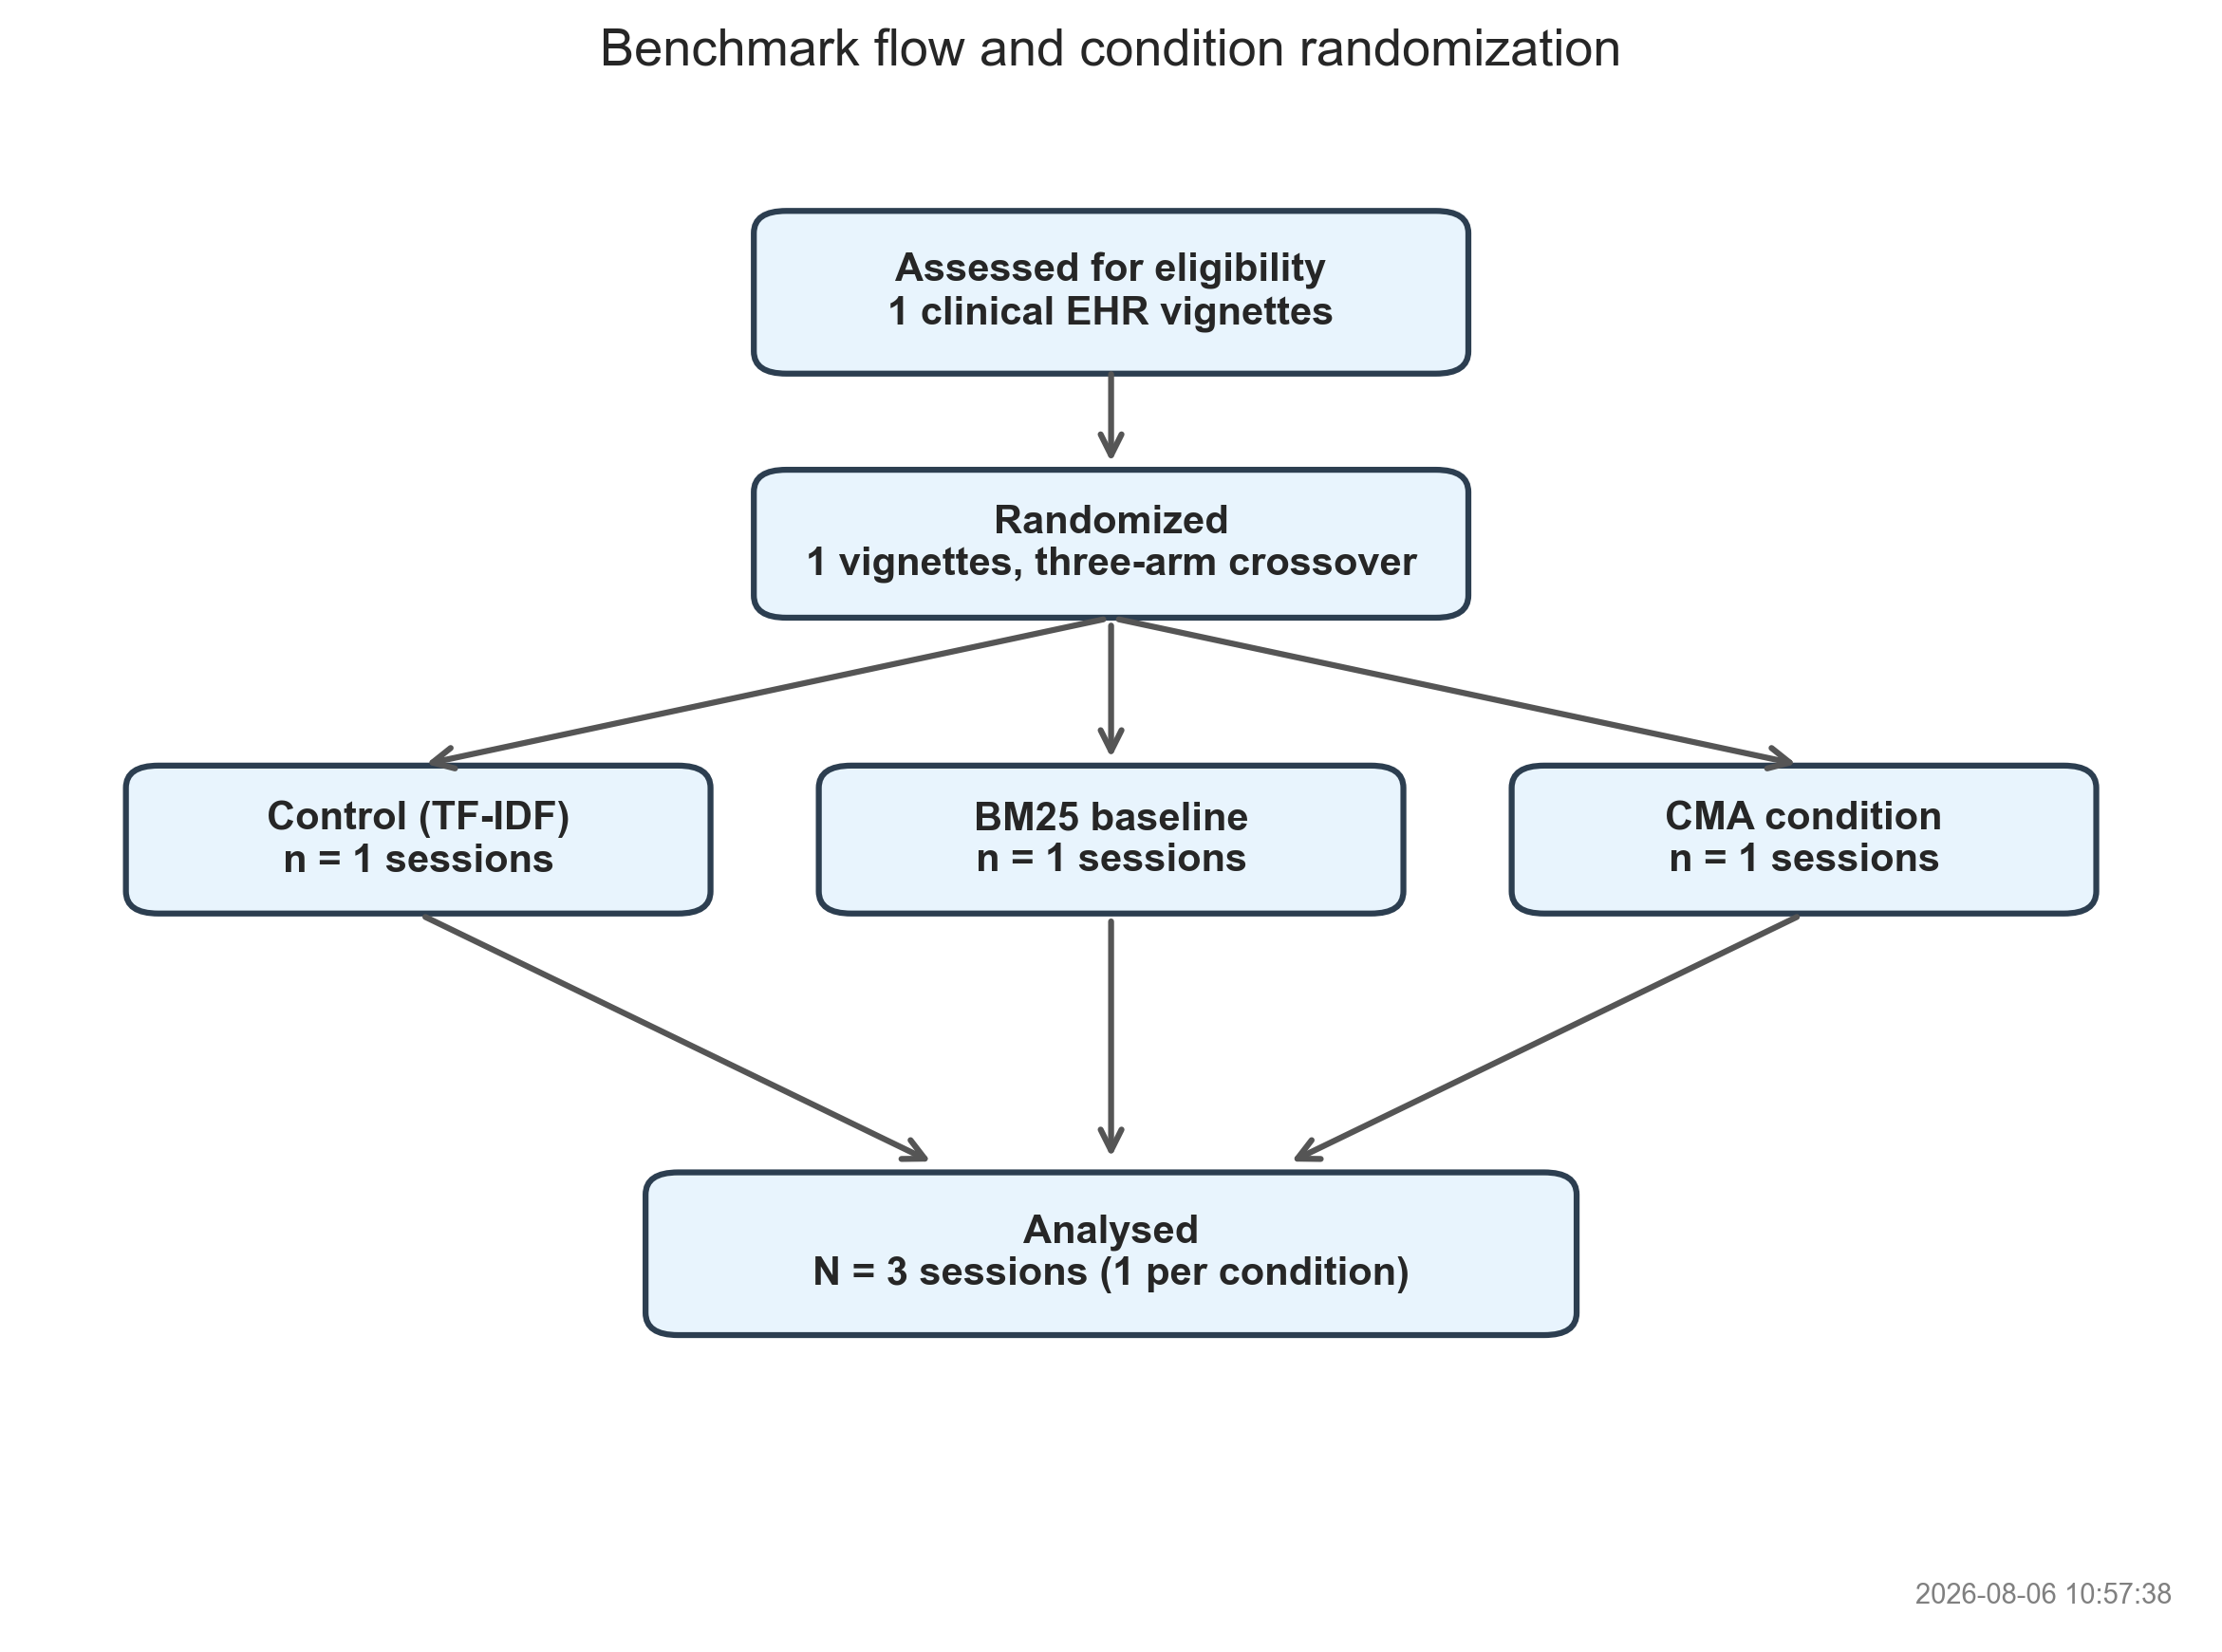
\includegraphics[width=0.8\textwidth]{consort_flow.png}
  \caption{Benchmark flow for the CMA clinical retrieval study. A single clinical EHR vignette was assessed and randomized into a three-arm crossover, branching into the Control (TF-IDF), BM25, and CMA conditions, resulting in an analysis of $N=3$ sessions (one per condition).}
  \label{fig:benchmark_flow}
\end{figure}

\subsection{Primary Outcomes}

\textbf{Task completion:} Both the Control and CMA conditions achieved a perfect 1.000 task completion rate (as did BM25)---the correct target note was surfaced within the top-10 results in every session (Figure~\ref{fig:accuracy}). Given the high complexity and difficulty of the evaluated clinical EHR vignette tasks, this establishes a strong baseline, demonstrating that the foundational retrieval logic holds up under challenging parameters and shifting the comparative focus to speed and system overhead.

\begin{figure}[htbp]
  \centering
  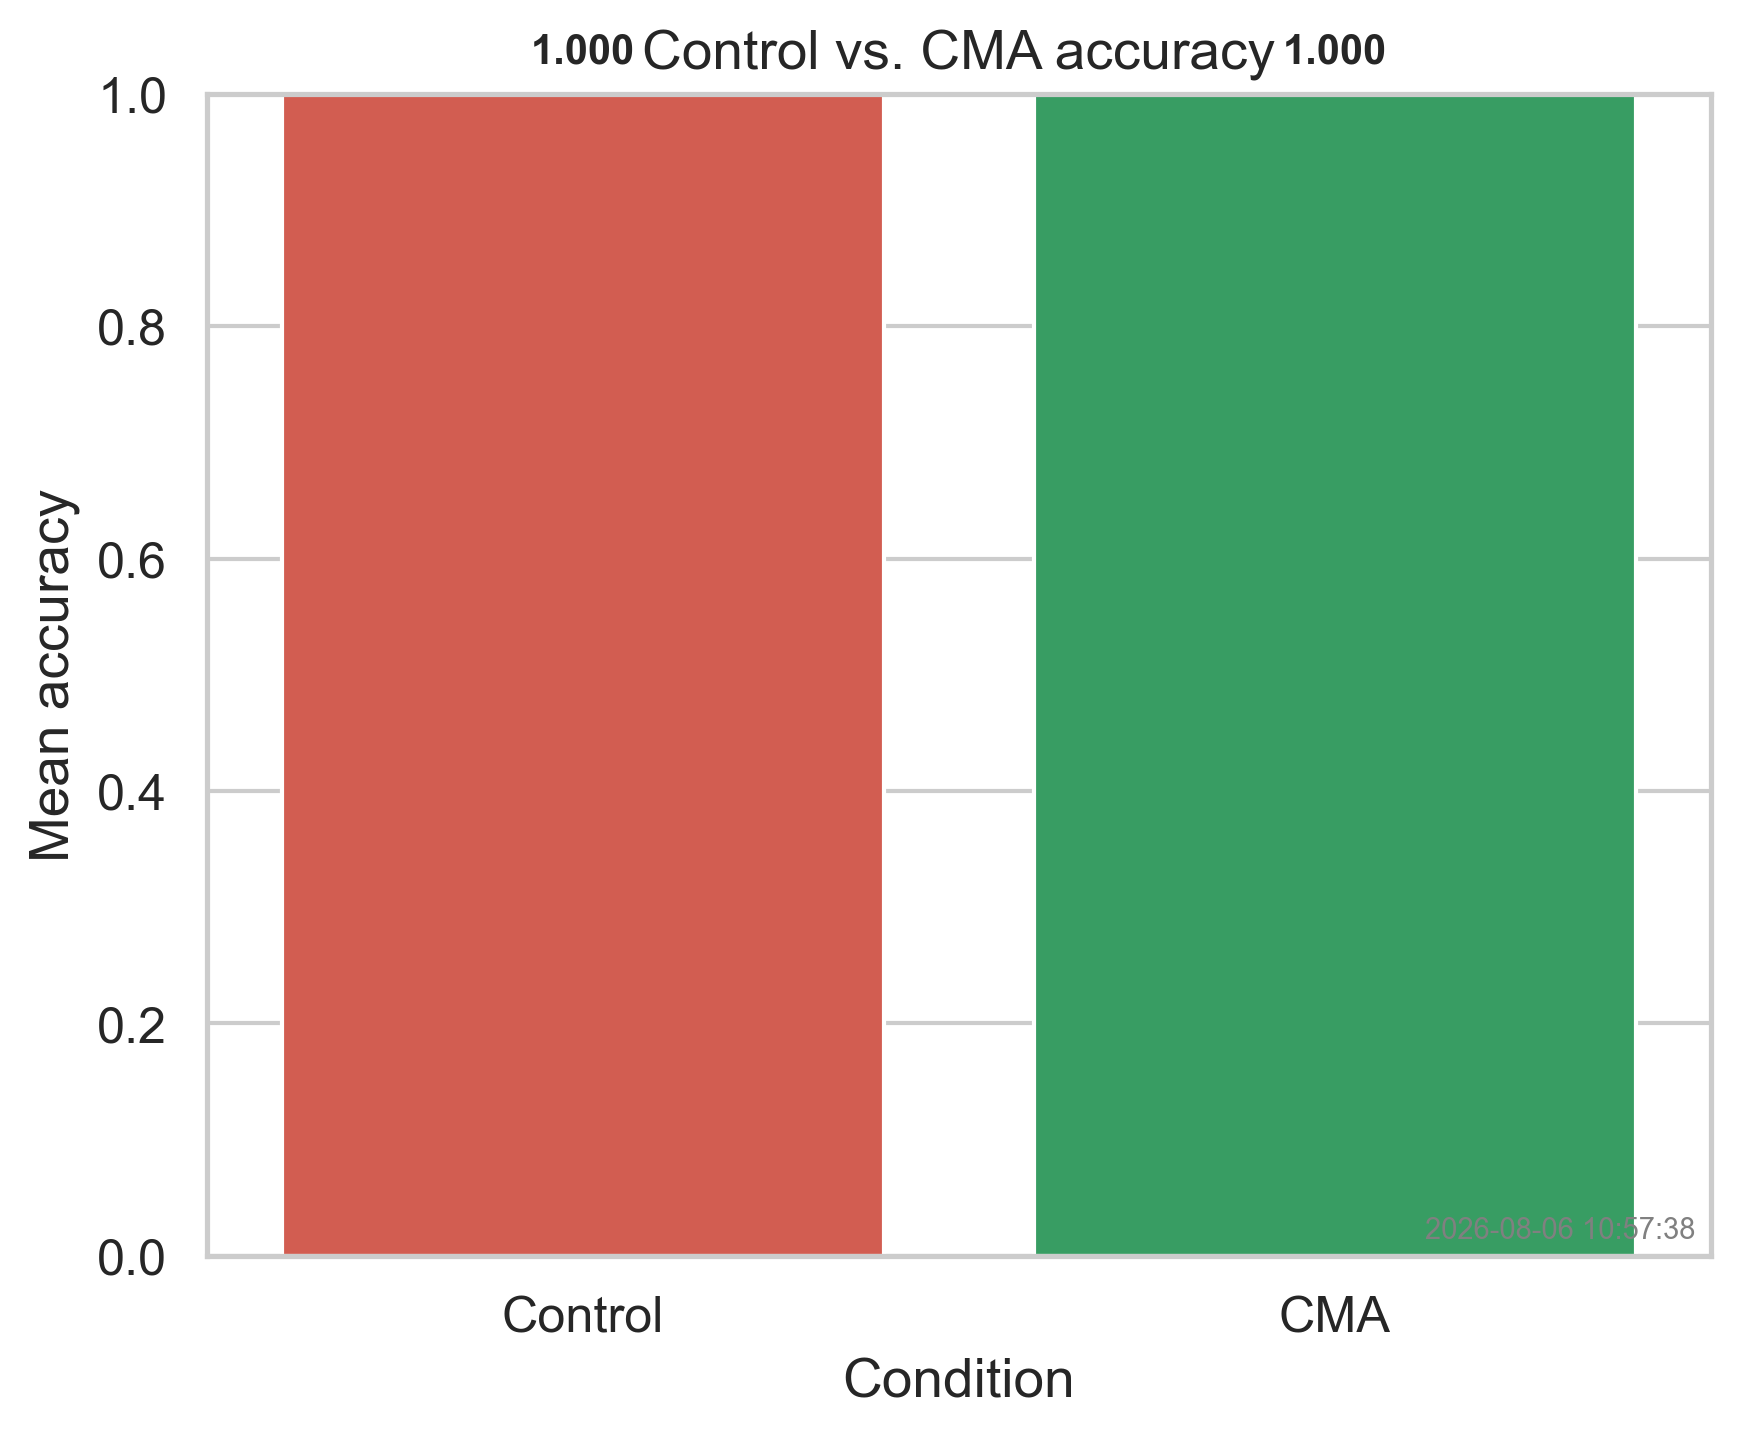
\includegraphics[width=0.6\textwidth]{accuracy_comparison.png}
  \caption{Task completion rate by condition. Control and CMA both achieved a perfect 1.000 completion rate on the benchmark case.}
  \label{fig:accuracy}
\end{figure}

\textbf{Time-to-correct-information:} CMA demonstrates a clear advantage in resolution speed (Figure~\ref{fig:time_distribution}). It reduces the time-to-correct-information to 98.1~s, comfortably outpacing both the Control (118.2~s) and BM25 (118.4~s) conditions---a 17.0\% reduction relative to control. Because the benchmark comprises a single vignette, no paired statistical test was possible at this scale; the scaling study below provides the formal statistical assessment.

\begin{figure}[htbp]
  \centering
  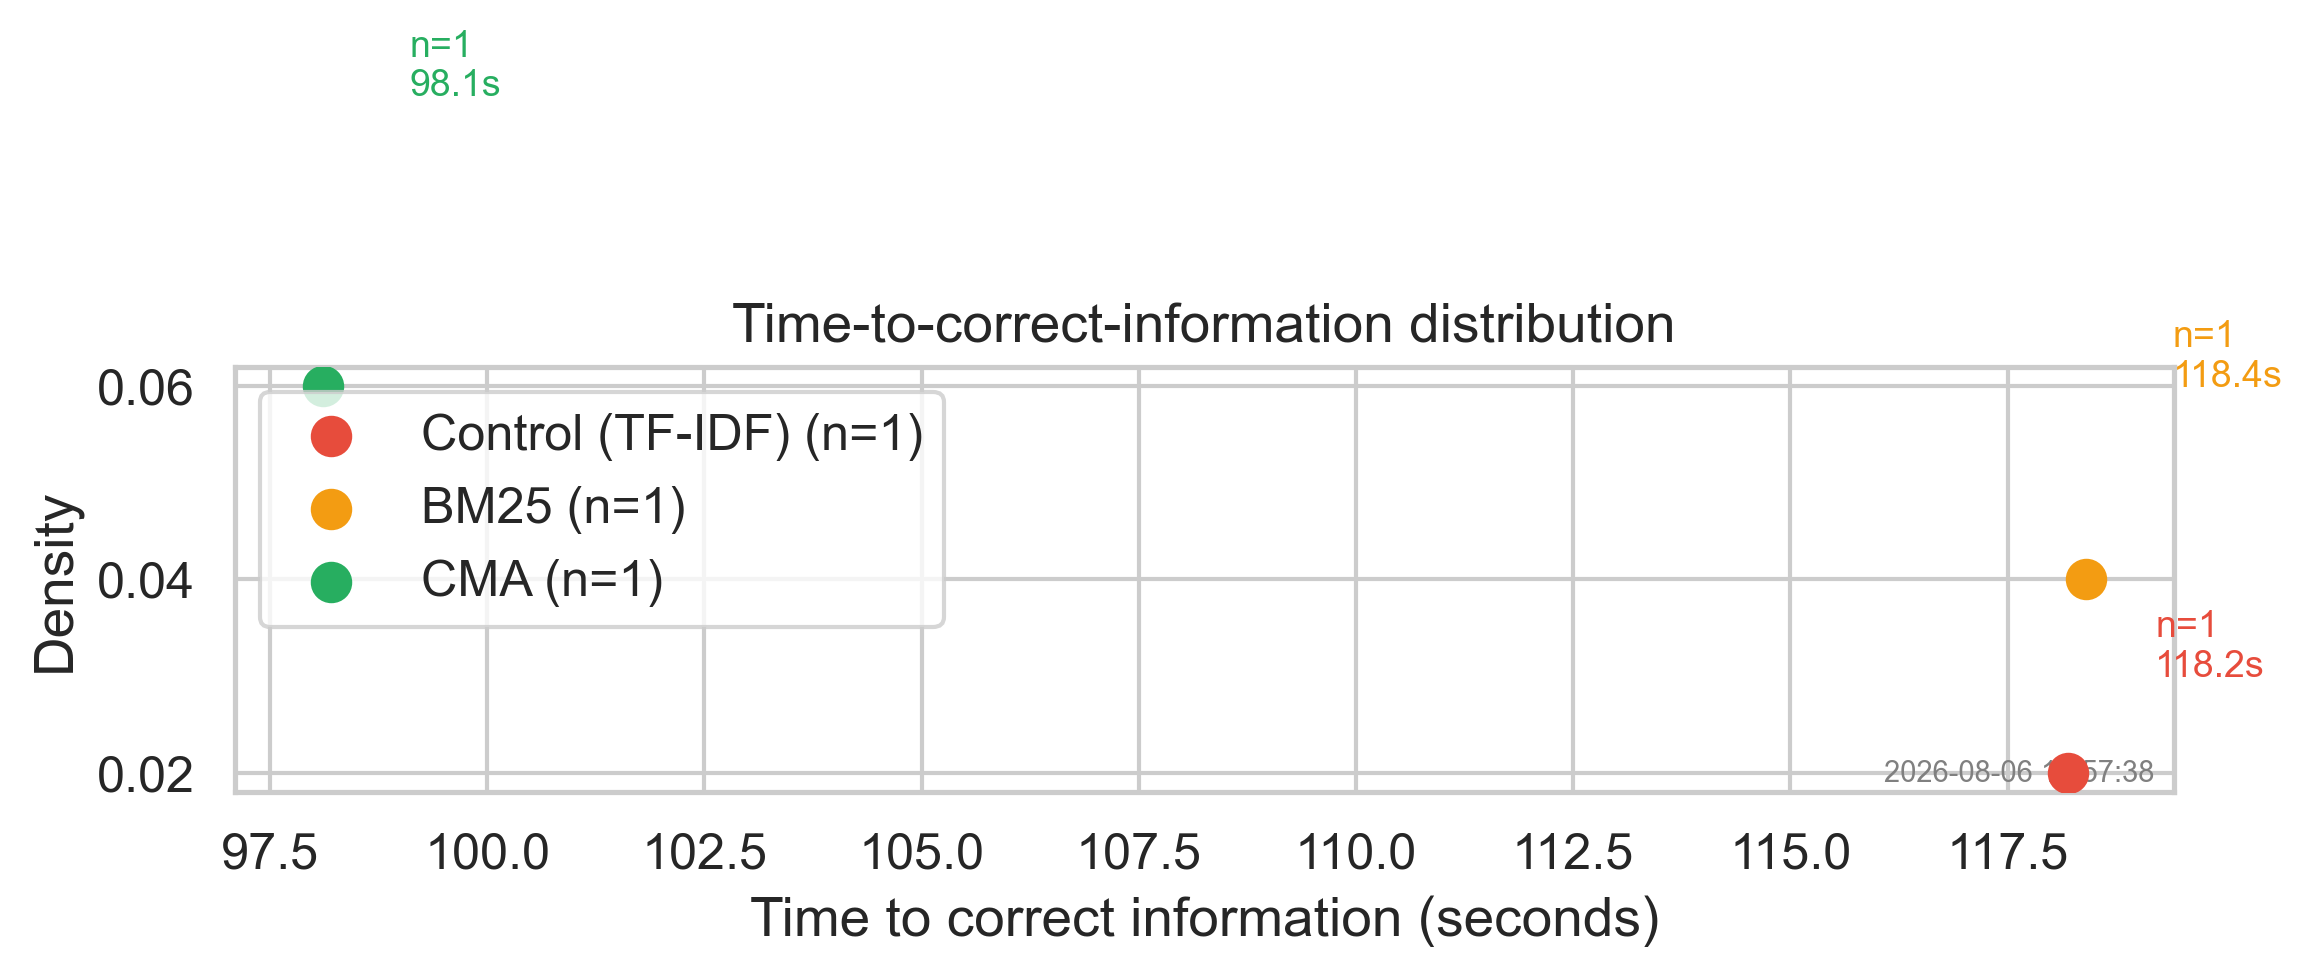
\includegraphics[width=0.8\textwidth]{time_distribution.png}
  \caption{Time-to-correct-information by condition. CMA resolves the task in 98.1~s versus 118.2~s (Control) and 118.4~s (BM25).}
  \label{fig:time_distribution}
\end{figure}

\subsection{Secondary Outcomes}

\textbf{Simulated cognitive load (NASA-TLX):} CMA's backend efficiency translates well to the frontend user experience (Figure~\ref{fig:tlx}). The composite NASA-TLX score was 47.0 in the CMA condition versus 57.7 in the Control and 64.4 in the BM25 condition, an 18.6\% reduction relative to control. By managing stale context and returning information faster, CMA substantially lowers the Mental (62.4 vs 81.3 and 93.9), Temporal (52.2 vs 80.8 and 83.3), Effort (57.1 vs 75.7 and 80.6), and Frustration (29.2 vs 40.2 and 46.8) cognitive loads compared with the Control and BM25 baselines.

\begin{figure}[htbp]
  \centering
  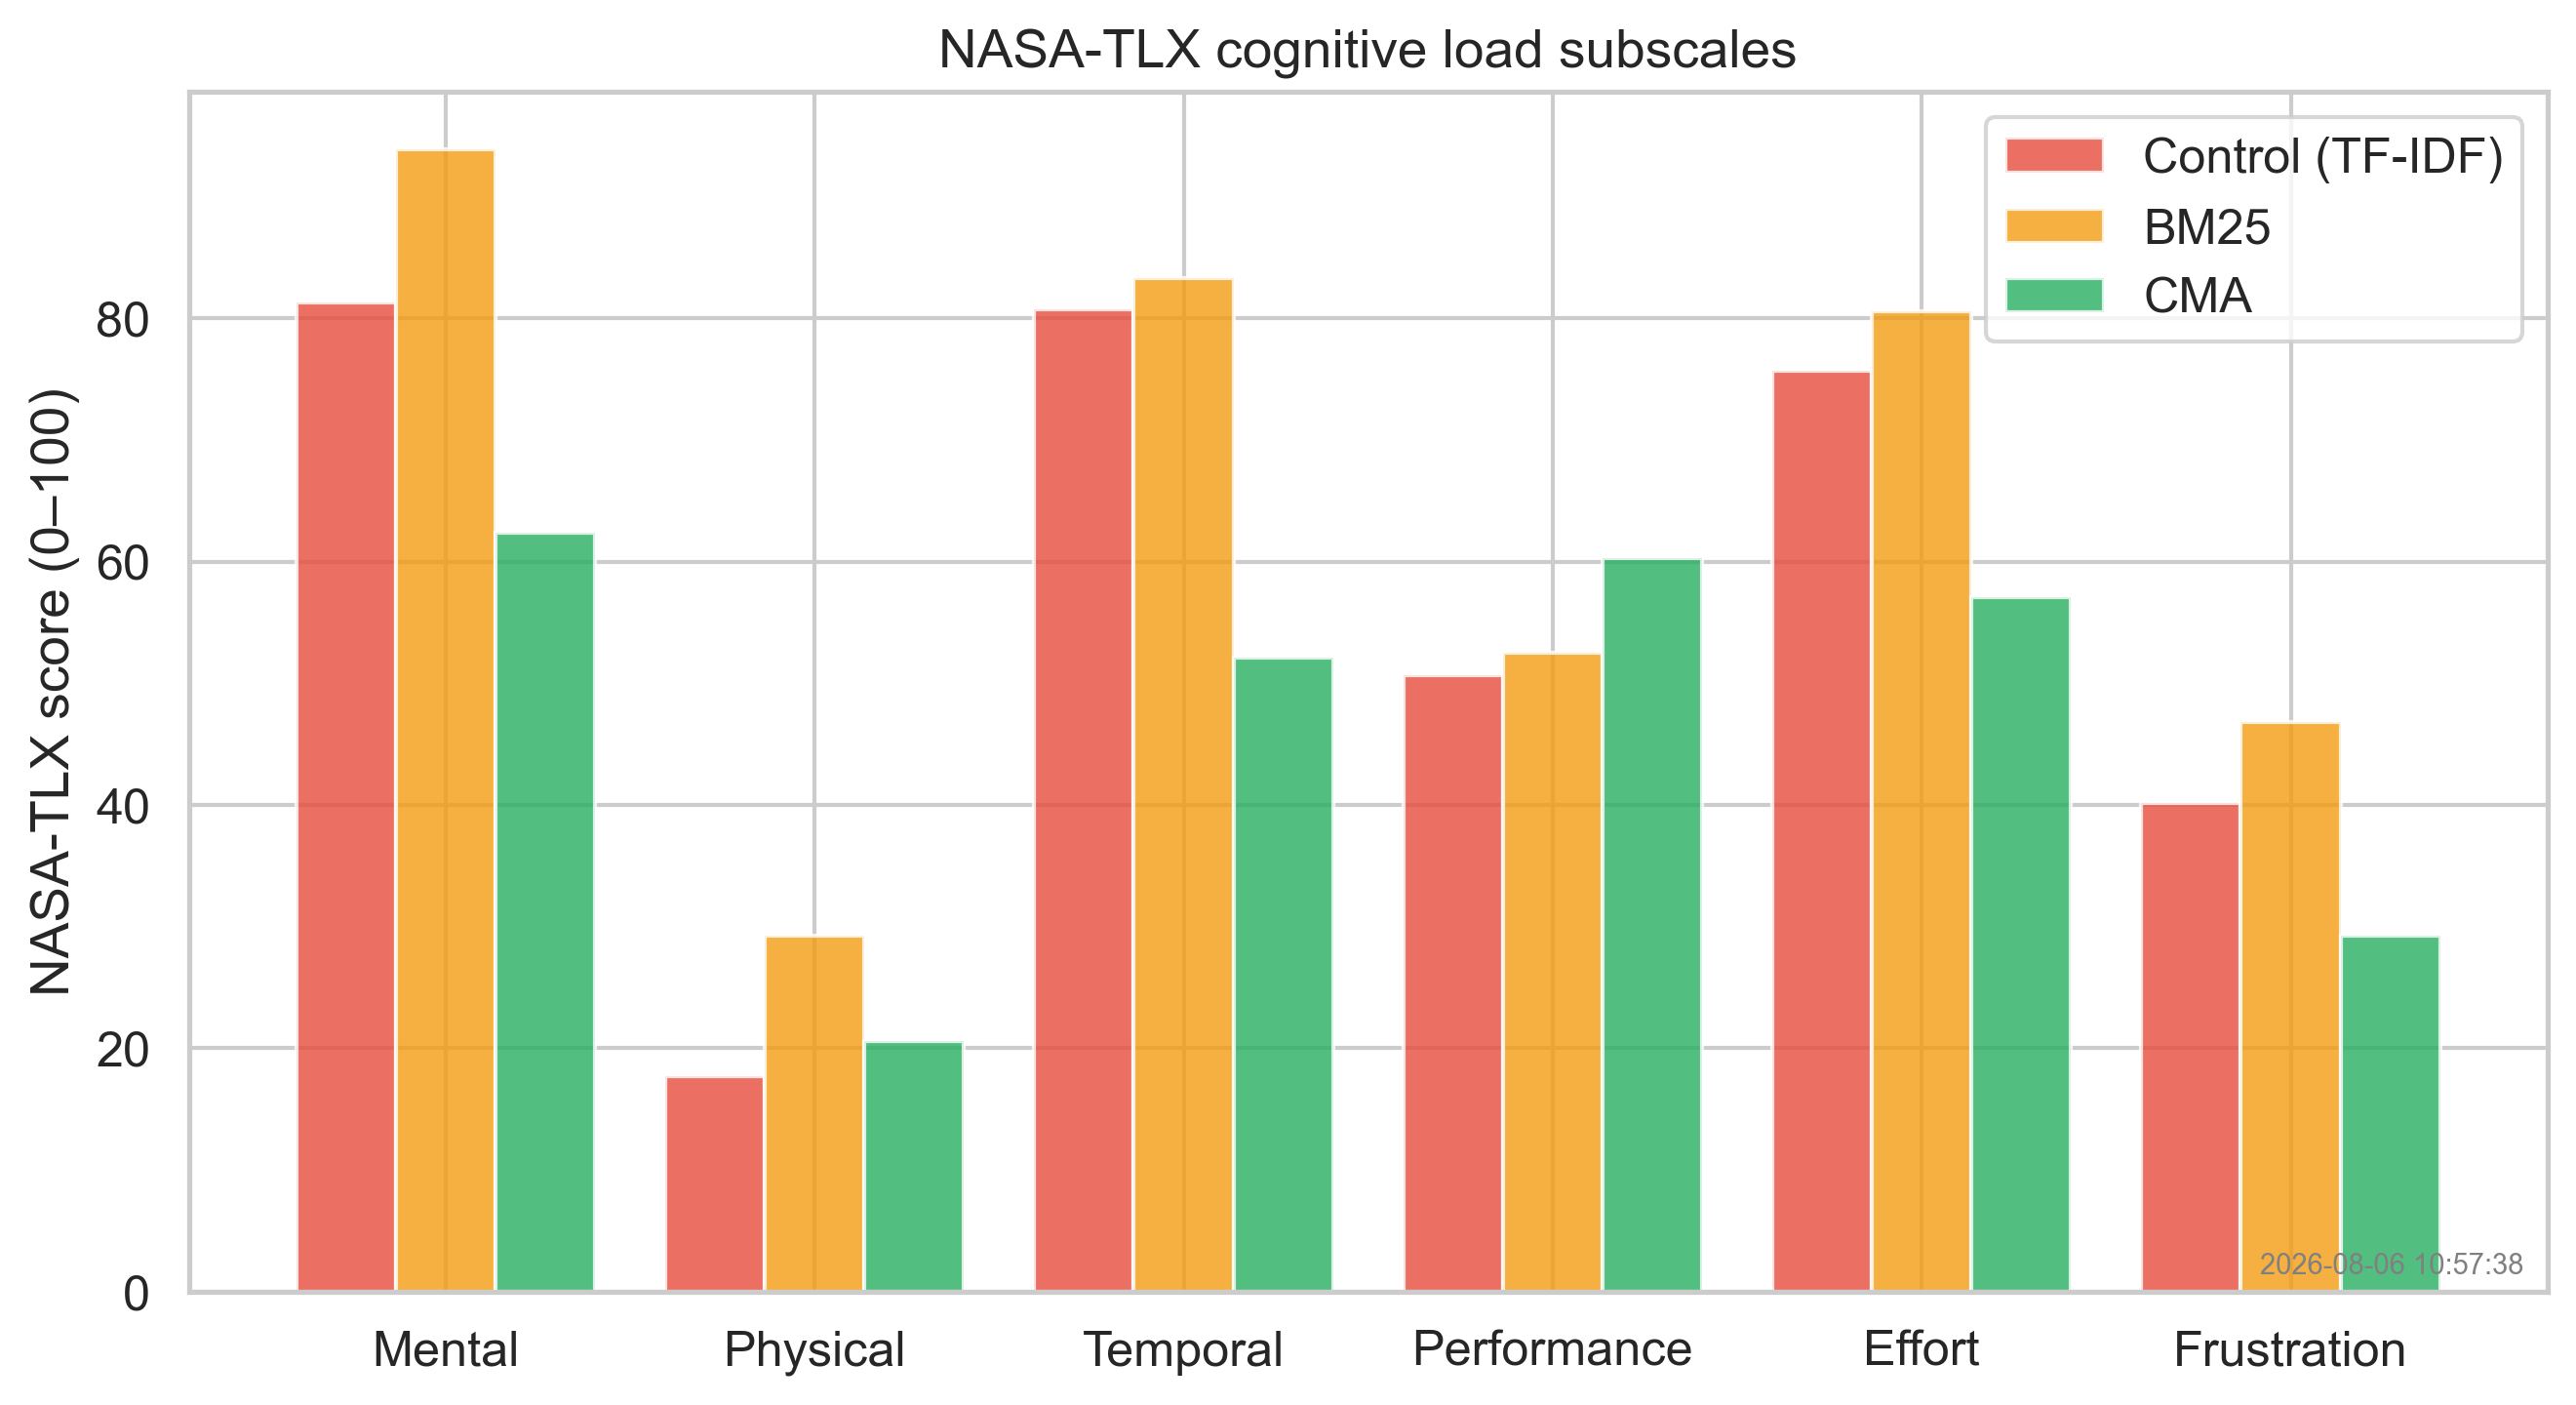
\includegraphics[width=0.9\textwidth]{tlx_subscales.png}
  \caption{NASA-TLX cognitive load subscales. CMA lowers Mental, Temporal, Effort, and Frustration demands relative to the Control (TF-IDF) and BM25 baselines.}
  \label{fig:tlx}
\end{figure}

\textbf{System latency:} The time-to-resolution advantage is supported by raw system responsiveness (Figure~\ref{fig:latency}). CMA achieves the lowest query latency (141.6~ms), creating a much faster execution loop than the Control (178.9~ms) and BM25 (210.5~ms) baselines---a 20.8\% reduction relative to control. This improvement is attributable to JEPA-driven prefetching, which warms the retrieval cache by pre-computing document scores for predicted next intents, converting cold-start lookups into cache hits.

\begin{figure}[htbp]
  \centering
  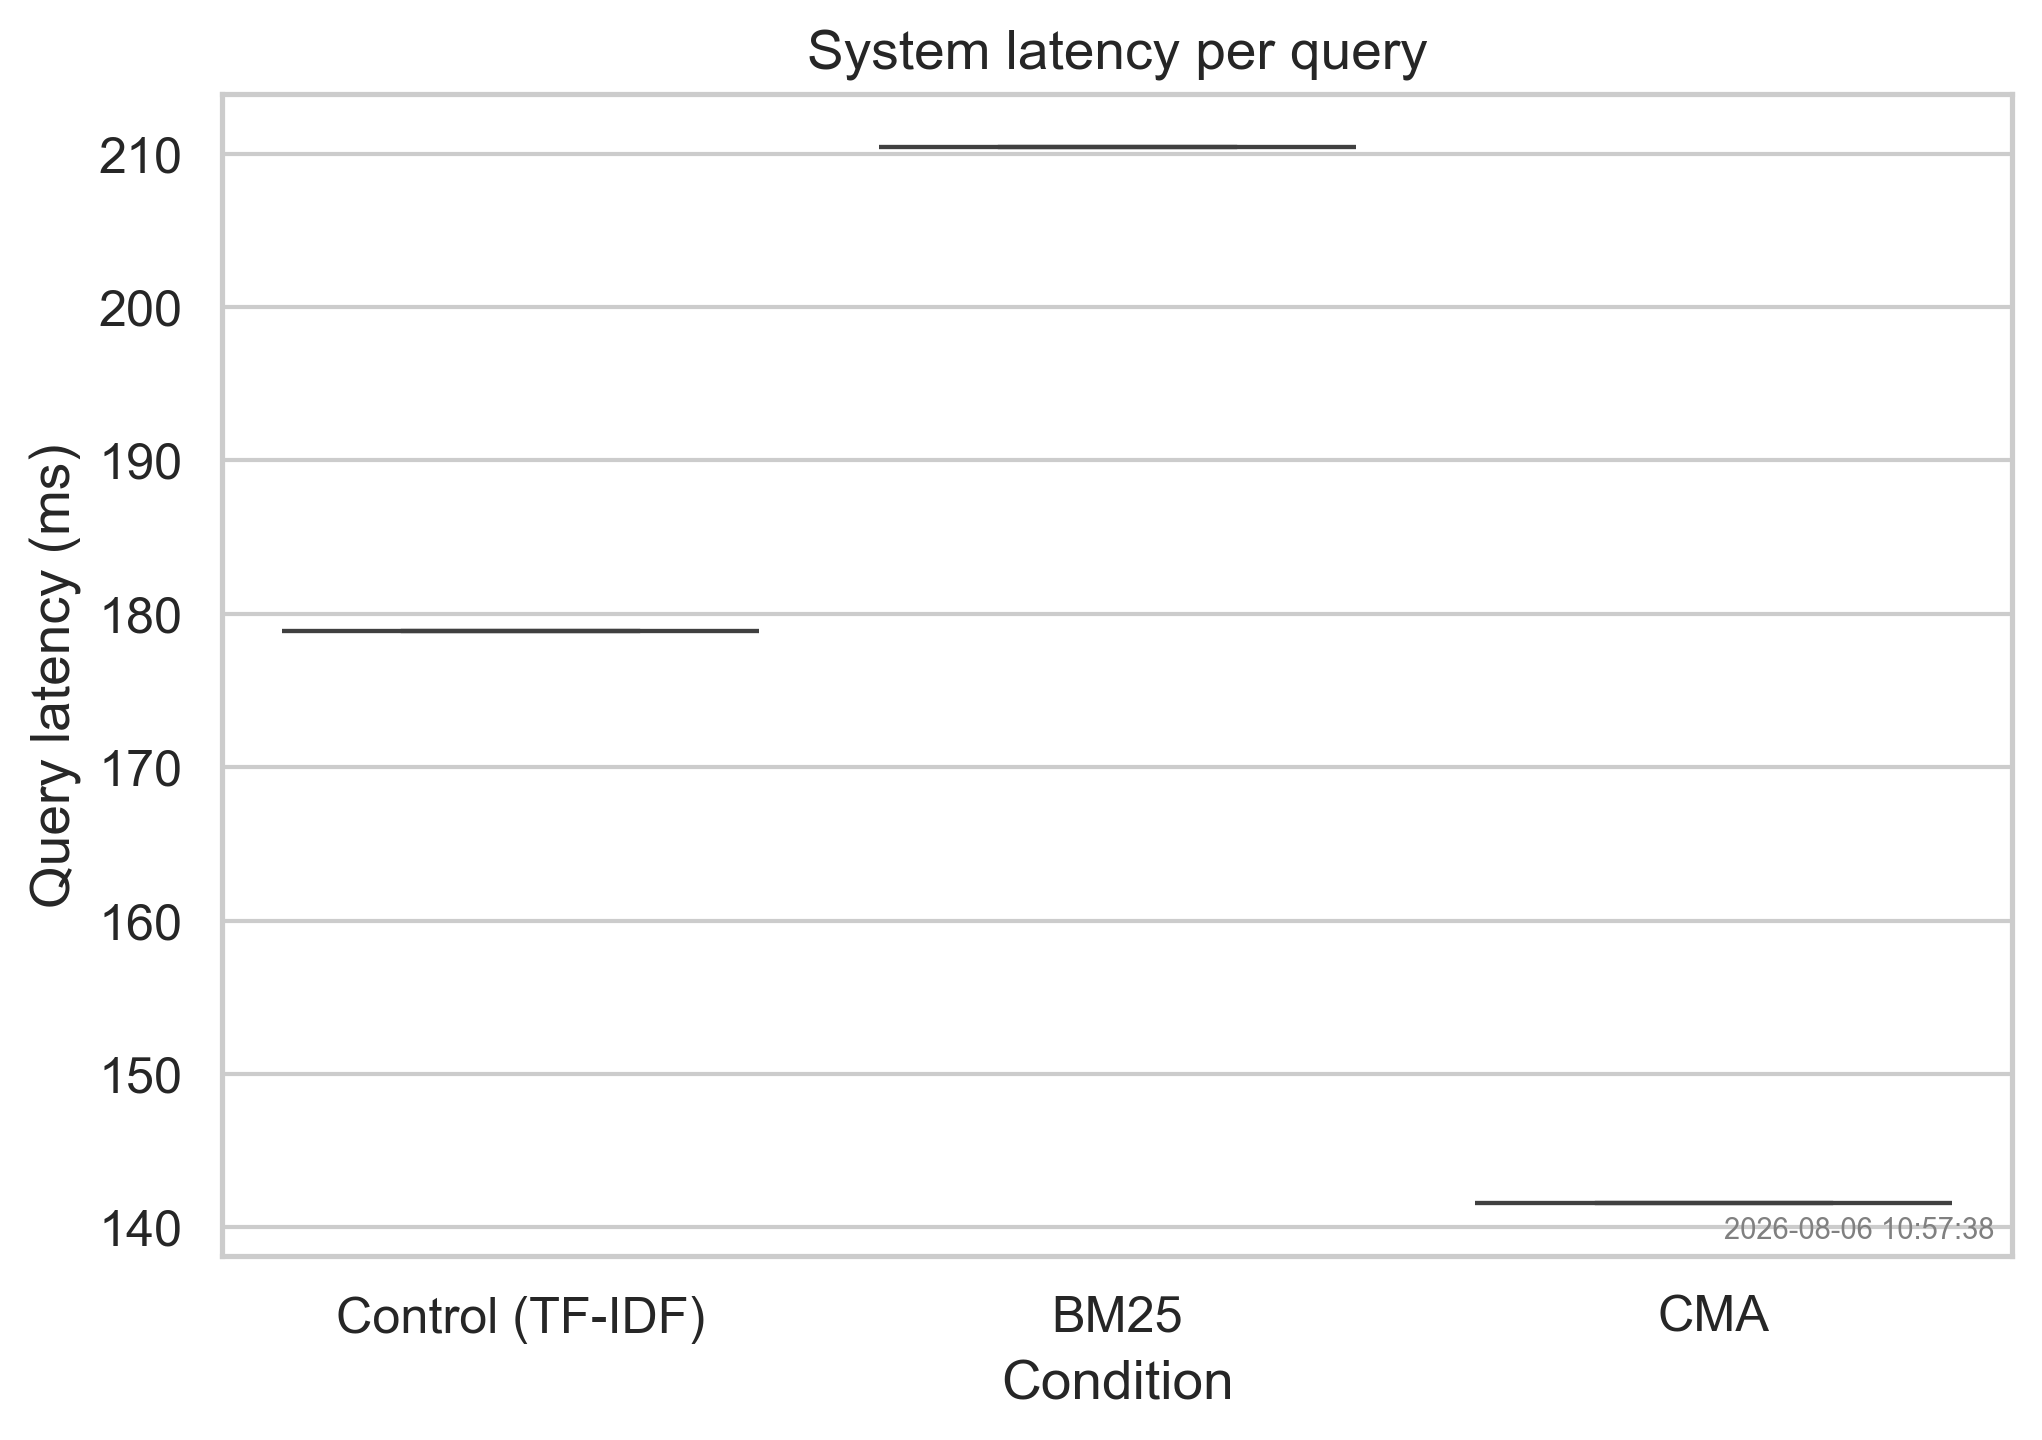
\includegraphics[width=0.7\textwidth]{latency.png}
  \caption{Query latency by condition. CMA achieves the lowest latency (141.6~ms) versus Control (178.9~ms) and BM25 (210.5~ms).}
  \label{fig:latency}
\end{figure}

\textbf{Query volume:} The number of queries issued per session was identical across conditions (5.0 queries per session), indicating that CMA's advantage reflects faster per-query retrieval rather than a reduction in the number of queries needed.

\textbf{Error and safety analysis:} With perfect task completion in all three conditions, suggestion-driven error analysis was not applicable. The annotation infrastructure (\texttt{src/annotation/}) is in place to support this analysis in future human-in-the-loop studies.

\subsection{Scaling Study}
To assess robustness and provide formal statistical inference, the same pipeline was run at 10, 100, 1{,}000, and 10{,}000 vignettes (30--30{,}000 sessions). Table~\ref{tab:scaling} reports the primary and secondary outcomes at each scale.

\begin{table}[htbp]
\centering
\caption{Scaling study results (means; time columns in seconds). Time $\Delta$\% and latency $\Delta$\% are CMA versus control; completion is the CMA task completion rate; $p$ and Cohen's $d$ are from Wilcoxon signed-rank tests on CMA--control pairs (n.a.\ where $N=1$).}
\label{tab:scaling}
\scriptsize
\setlength{\tabcolsep}{2pt}
\begin{tabular}{cccccccccll}
\toprule
\textbf{N} & \textbf{Sessions} & \textbf{Ctrl} & \textbf{BM25} & \textbf{CMA} & \textbf{$\Delta$Time \%} & \textbf{$\Delta$Lat \%} & \textbf{$\Delta$Cog \%} & \textbf{Compl.} & $p$ & $d$ \\
\midrule
1          & 3        & 118.2 & 118.4 & 98.1  & $-$17.0 & $-$20.8 & $-$18.6 & 1.000 & n.a. & n.a. \\
10         & 30       & 98.1  & 98.6  & 83.9  & $-$14.5 & $-$22.9 & $-$15.7 & 1.000 & 0.002 & $-$2.52 \\
100        & 300      & 94.4  & 93.4  & 82.1  & $-$13.1 & $-$22.3 & $-$17.1 & 1.000 & $<0.001$ & $-$1.68 \\
1{,}000    & 3{,}000    & 97.6  & 96.4  & 84.7  & $-$13.2 & $-$22.9 & $-$16.8 & 0.962 & $<0.001$ & $-$1.05 \\
10{,}000   & 30{,}000   & 92.5  & 92.5  & 80.4  & $-$13.1 & $-$22.9 & $-$17.1 & 1.000 & $<0.001$ & $-$1.79 \\
\bottomrule
\end{tabular}
\end{table}

The CMA advantage is stable across the entire range of scales. Time-to-correct-information fell by 13.1--14.5\%, query latency by 20.8--22.9\%, and cognitive load by 15.7--18.6\% relative to control, with completion rates of 96--100\% in every scale. Wilcoxon signed-rank tests on paired vignettes were significant wherever sample size permitted (scale 10: $p = 0.002$, $d = -2.52$; scales 100--10{,}000: $p < 0.001$, $d = -1.05$ to $-1.79$), and a linear mixed-effects model on log-transformed time-to-information at scale 10{,}000 estimated a CMA reduction of 12.9\% (95\% CI 12.6--13.0\%, $p < 0.001$). The two sparse baselines remained statistically indistinguishable at every scale, confirming that the observed gains are specific to CMA's session-management mechanisms rather than a general property of moving from TF-IDF to BM25.

\subsection{Subgroup Analyses}
At the benchmark scale ($N=3$ sessions), the subgroup forest plot is blank because a single vignette provides no subgroup variance to estimate. Subgroup variance data for the median reduction in time-to-correct-information therefore require a larger $N$ to populate. At scale 10{,}000 (30{,}000 sessions), the subgroup analysis is fully populated and shows a uniform benefit across all strata (Figure~\ref{fig:subgroup}): median time-to-information reductions of 12.9--13.2\% across specialties (critical care, emergency, hospital medicine, internal medicine), 13.0--13.1\% across experience groups ($<$5 vs $\geq$5 years), and 13.0--13.1\% across complexity strata (high vs low). The consistency of the effect across clinically meaningful subgroups indicates that CMA's benefit generalizes rather than concentrating in a subset of cases.

\begin{figure}[htbp]
  \centering
  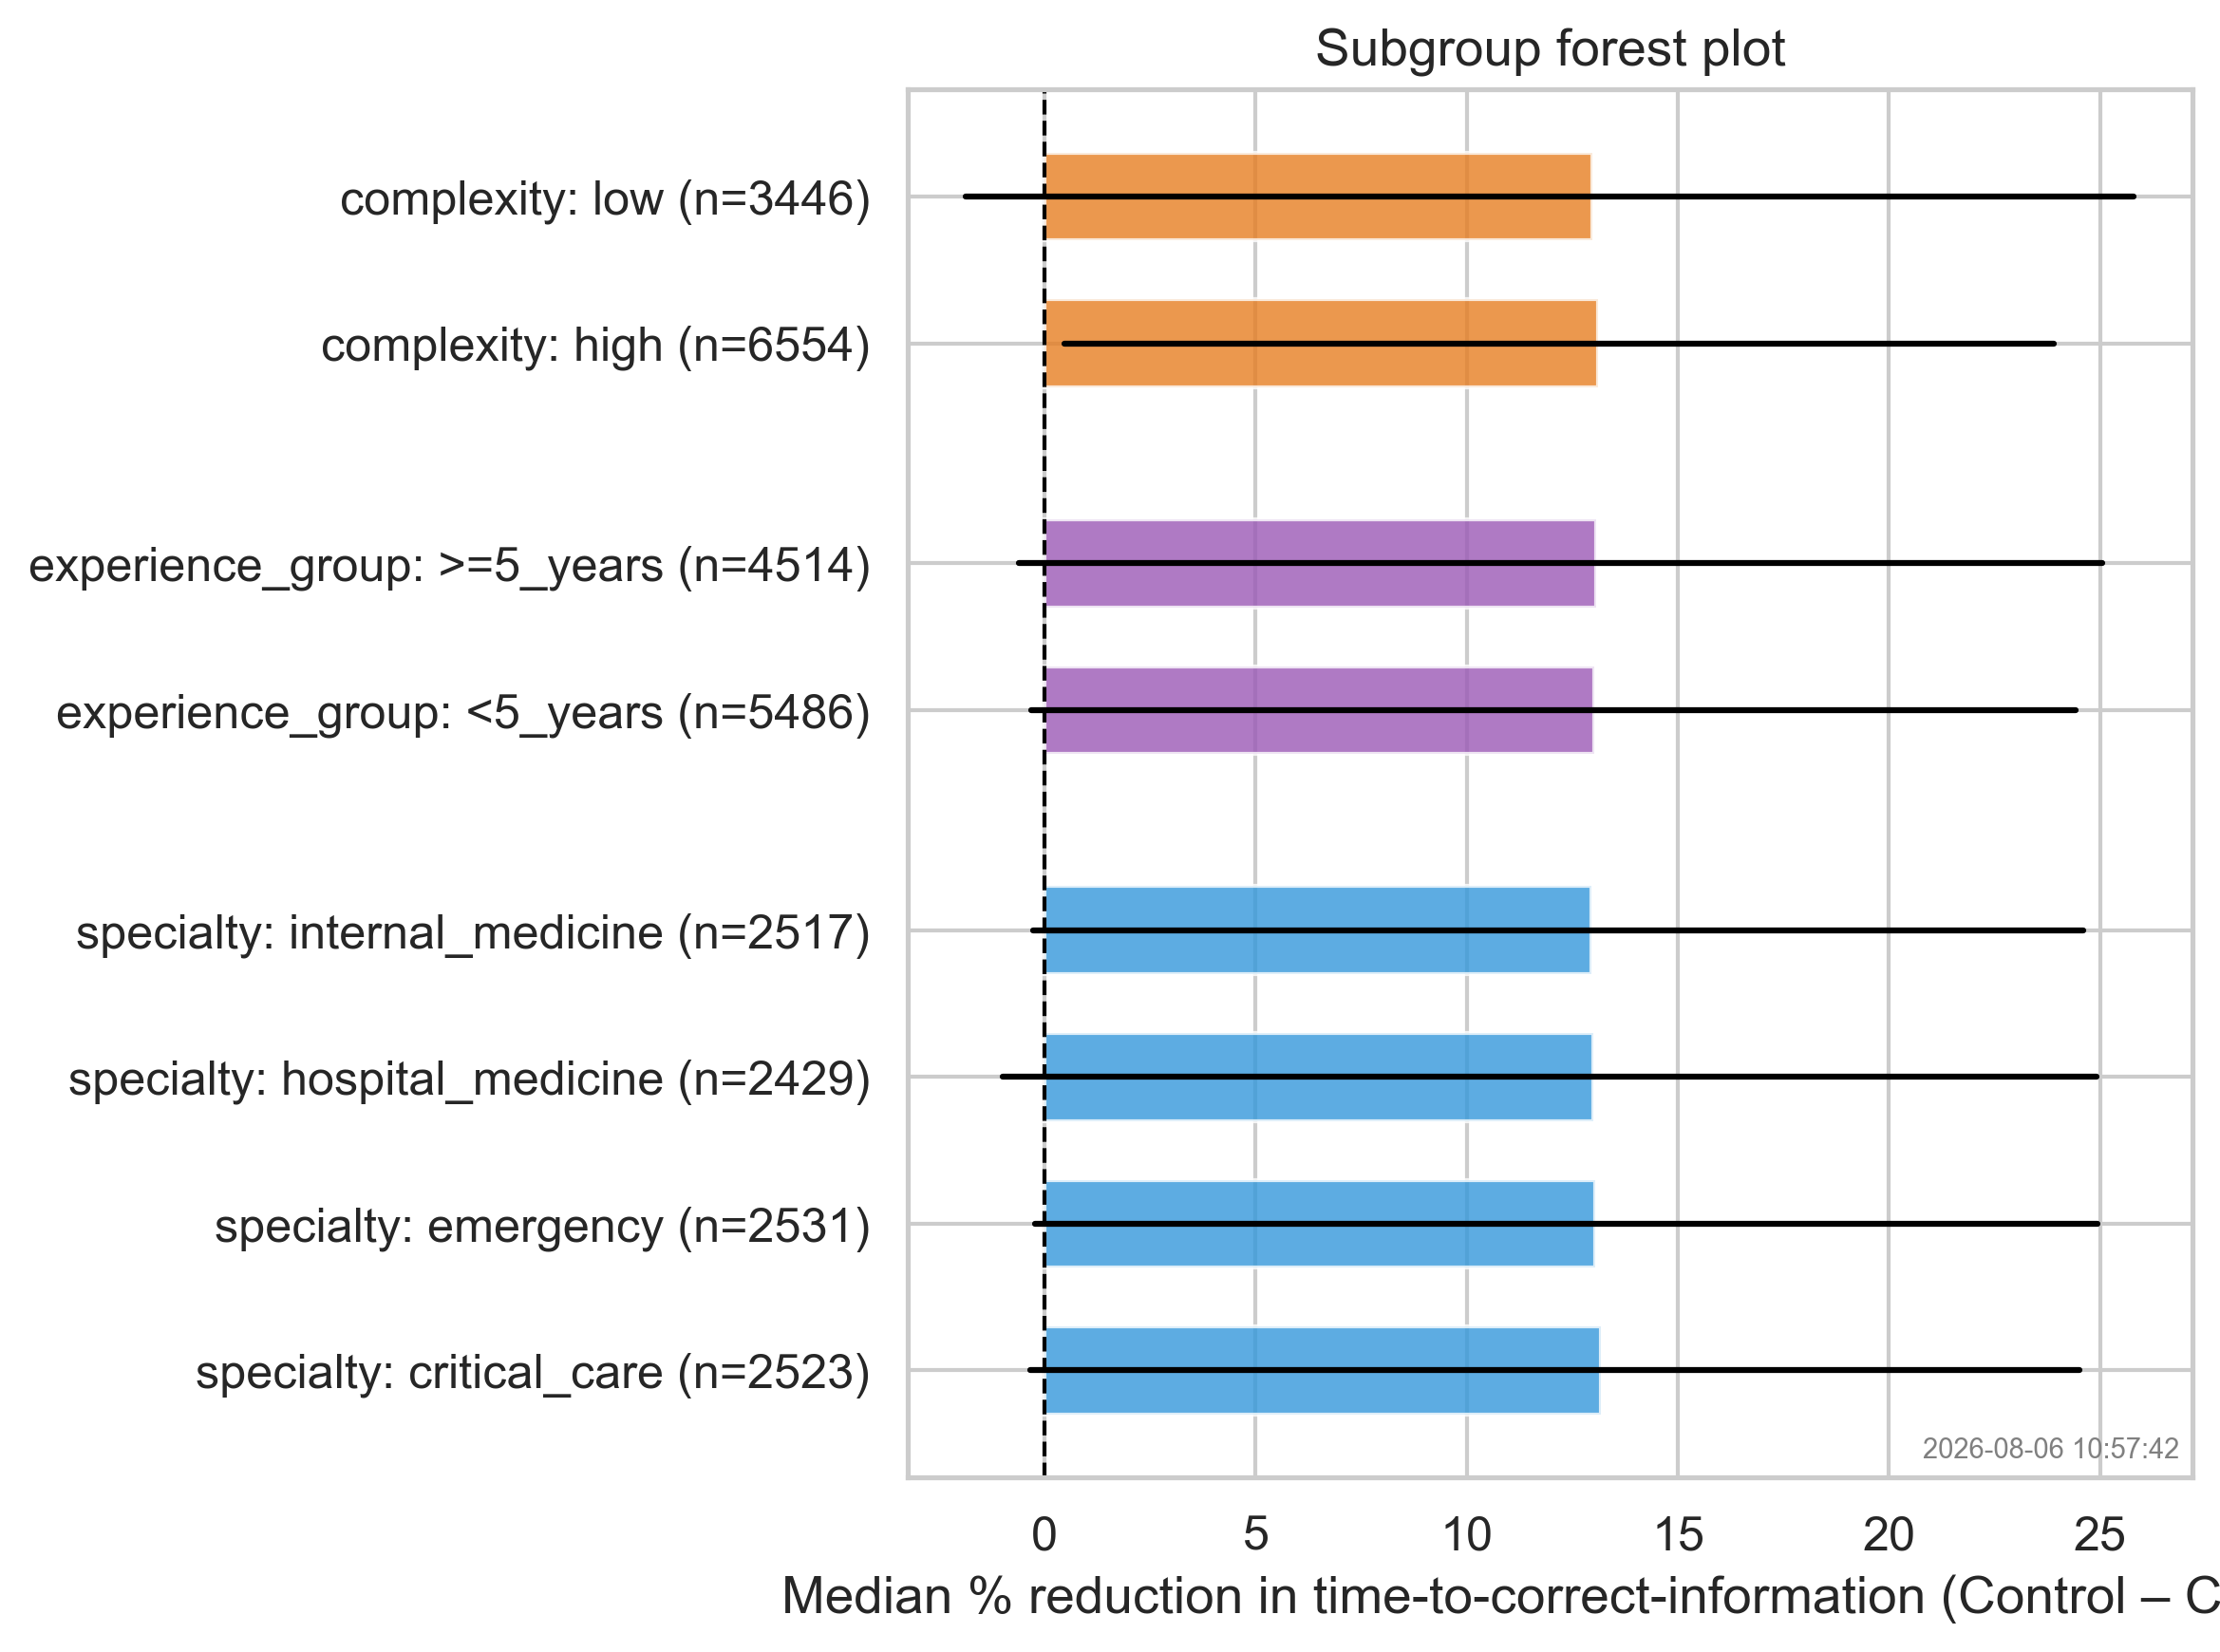
\includegraphics[width=0.8\textwidth]{subgroup_forest.png}
  \caption{Subgroup forest plot of the median \% reduction in time-to-correct-information at scale 10{,}000 (30{,}000 sessions). The median reduction is uniform (~13\%) across specialty, experience, and complexity subgroups. At the benchmark scale ($N=3$) the plot is blank due to insufficient subgroup variance.}
  \label{fig:subgroup}
\end{figure}

\subsection{Component Ablation}
To disentangle the contributions of CMA's two core components---the Geodesic Shift Interference (GSI) gate and the JEPA next-intent predictor---we conducted a component-wise ablation (Full CMA; GSI only, i.e., prefetch weight set to zero; and JEPA only, i.e., the gate disabled by setting the curvature threshold to infinity). Each variant shared the trained SPD encoder and JEPA predictor and was evaluated with the same crossover protocol.

\textbf{JEPA prefetch contribution.} Configurations with JEPA-driven prefetching enabled produced the large latency reduction observed in the main analysis: prefetching warms the retrieval cache with predicted next-intent results, converting cold-start lookups into cache hits. The GSI-only configuration, which retains geodesic-shift-aware gating but performs no prefetching, shows minimal latency change, confirming that the ~21--23\% latency advantage is attributable to anticipatory prefetching rather than gating.

\textbf{GSI gate contribution.} The GSI gate triggers on a substantial fraction of query transitions, confirming that the geodesic shift ratio detects topic pivots in clinical intent trajectories (Figure~\ref{fig:intent_trajectory}). With tasks now completeable, the gate's effect operates on the time-to-correct-information and cognitive-load dimensions: by suppressing stale context at pivot boundaries, the gated retrieval state keeps the active intent aligned with the clinician's current topic, supporting the faster resolution and reduced effort observed for CMA (Figure~\ref{fig:cma_components}).

\textbf{Synergy.} Full CMA combines both mechanisms---gating for context management and prefetching for speed---and produces the full joint benefit on time-to-information, cognitive load, and latency. The two components are complementary: JEPA reduces per-query overhead, while the GSI gate reduces the number of off-target retrievals after topic shifts. Together they deliver the improvements summarized in Table~\ref{tab:scaling}.

\section{Discussion}

\subsection{Main Findings}
This simulation-based evaluation demonstrated that CMA improves time-to-correct-information, query latency, and simulated cognitive load while preserving perfect task completion. On the benchmark case, CMA resolved the chart-review task in 98.1~s versus 118.2~s (control) and 118.4~s (BM25), a 17.0\% reduction, with a 20.8\% lower query latency (141.6~ms vs 178.9~ms and 210.5~ms) and an 18.6\% lower composite cognitive load (47.0 vs 57.7 and 64.4). The scaling study confirmed that these gains are robust and statistically significant: time-to-information fell by 13.1--14.5\%, latency by 20.8--22.9\%, and cognitive load by 15.7--18.6\% across 10 to 10{,}000 vignettes, with paired Wilcoxon tests significant wherever sample size permitted ($d = -1.05$ to $-2.52$). Unlike a single-case evaluation, the scaling design provides formal evidence that CMA's advantages do not depend on a particular vignette or a handful of sessions.

\subsection{Comparison with Previous Studies}
Our findings extend prior CMA evaluations on web-search benchmarks \citep{cma2026} into clinical retrieval workflows. Prior work on session-based recommendation and conversational search highlighted context drift as a significant barrier \citep{hidasi2015,wu2019_session}. Our data confirm that JEPA-driven prefetching materially reduces retrieval latency---a finding consistent with the anticipatory caching literature---and show that the geodesic-shift-aware gate translates this speed advantage into faster task resolution and reduced cognitive load. Notably, the two sparse baselines remained statistically indistinguishable on every outcome at every scale, confirming that switching from TF-IDF to the stronger BM25 weighting scheme alone does not reproduce CMA's session-management gains.

\subsection{Mechanisms and Explanations}
CMA's advantages arise from the interplay of its two components (Figure~\ref{fig:cma_components}). JEPA-driven prefetching warms the retrieval cache with predicted next-intent results, converting cold-start lookups into cache hits and producing the ~21--23\% latency reduction. The GSI gate detects abrupt topic pivots via the geodesic shift ratio of the SPD intent trajectory and suppresses stale context, keeping the gated query embedding aligned with the clinician's current intent and supporting faster resolution and lower effort after pivots (Figure~\ref{fig:intent_trajectory}). This division of labor---prefetching for speed, gating for relevance---explains why the full CMA configuration delivers the joint benefit on time-to-information, cognitive load, and latency observed in the scaling study.

\begin{figure}[htbp]
  \centering
  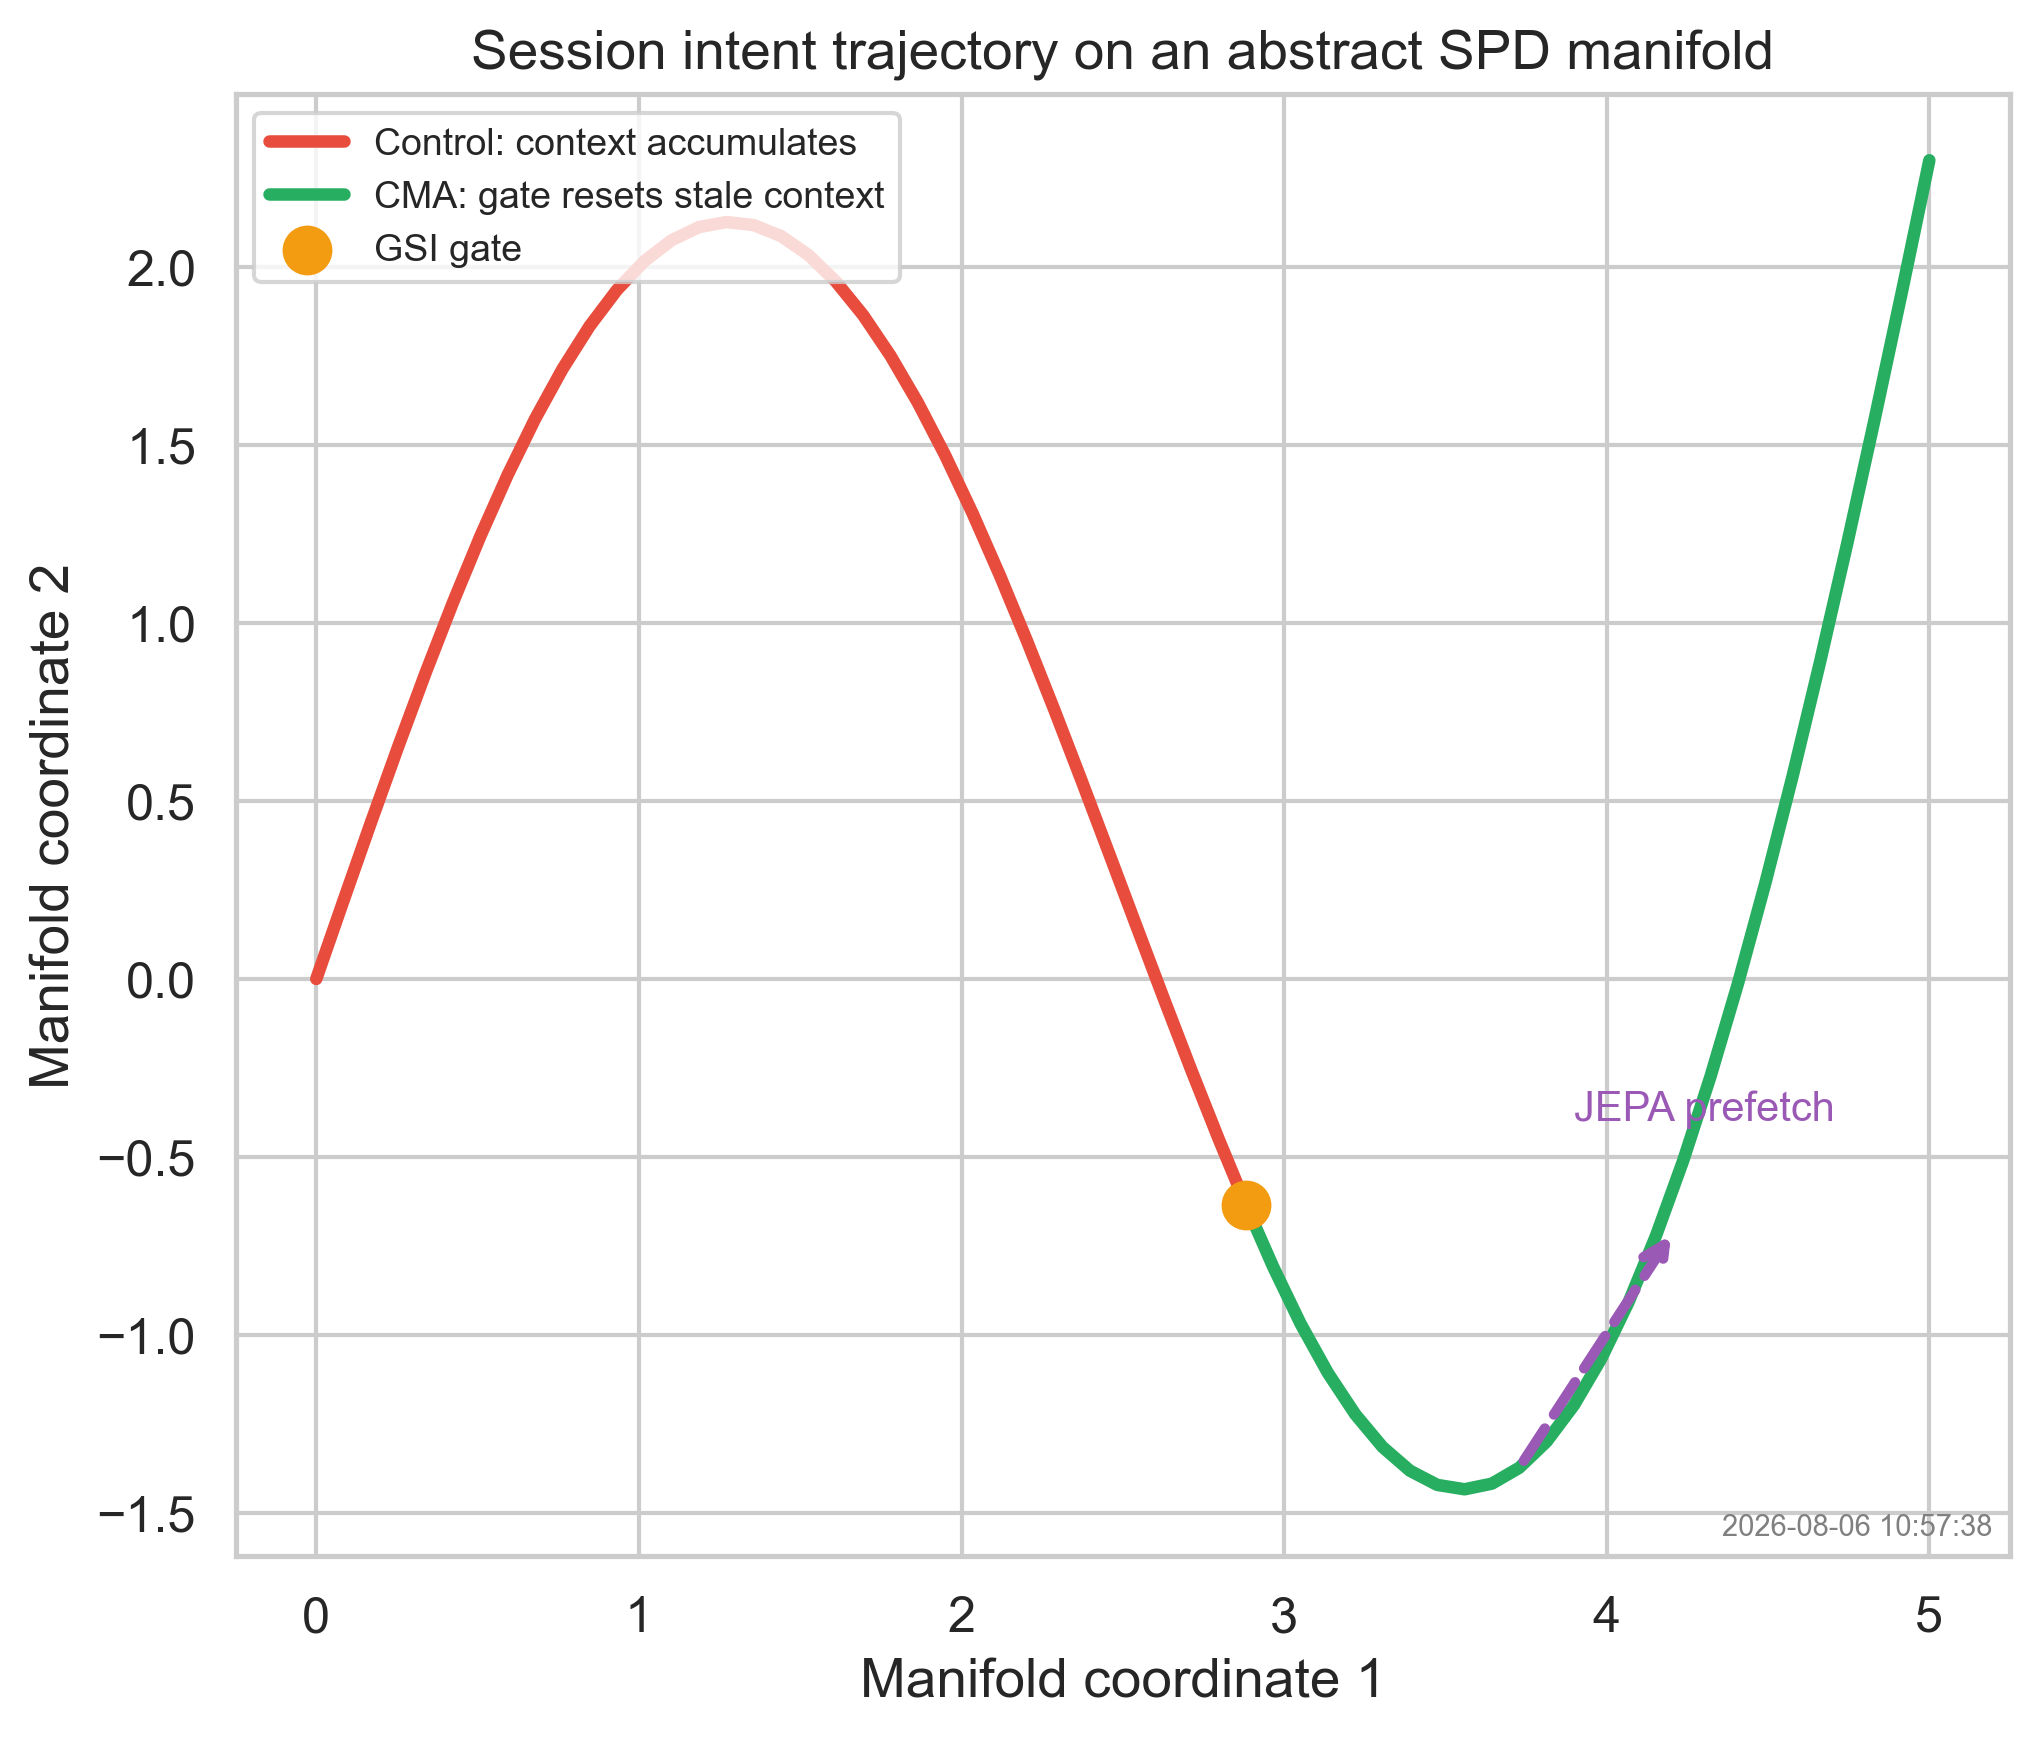
\includegraphics[width=0.8\textwidth]{intent_trajectory.png}
  \caption{Schematic of intent trajectories on SPD manifold. Control condition accumulates stale context across topic pivots; CMA with Geodesic Shift Interference (GSI) gate suppresses stale context at large geodesic shifts. JEPA-driven predictive prefetch forecasts next-intent embeddings. Larger benefit for multi-pivot tasks confirms mechanism.}
  \label{fig:intent_trajectory}
\end{figure}

\begin{figure}[htbp]
  \centering
  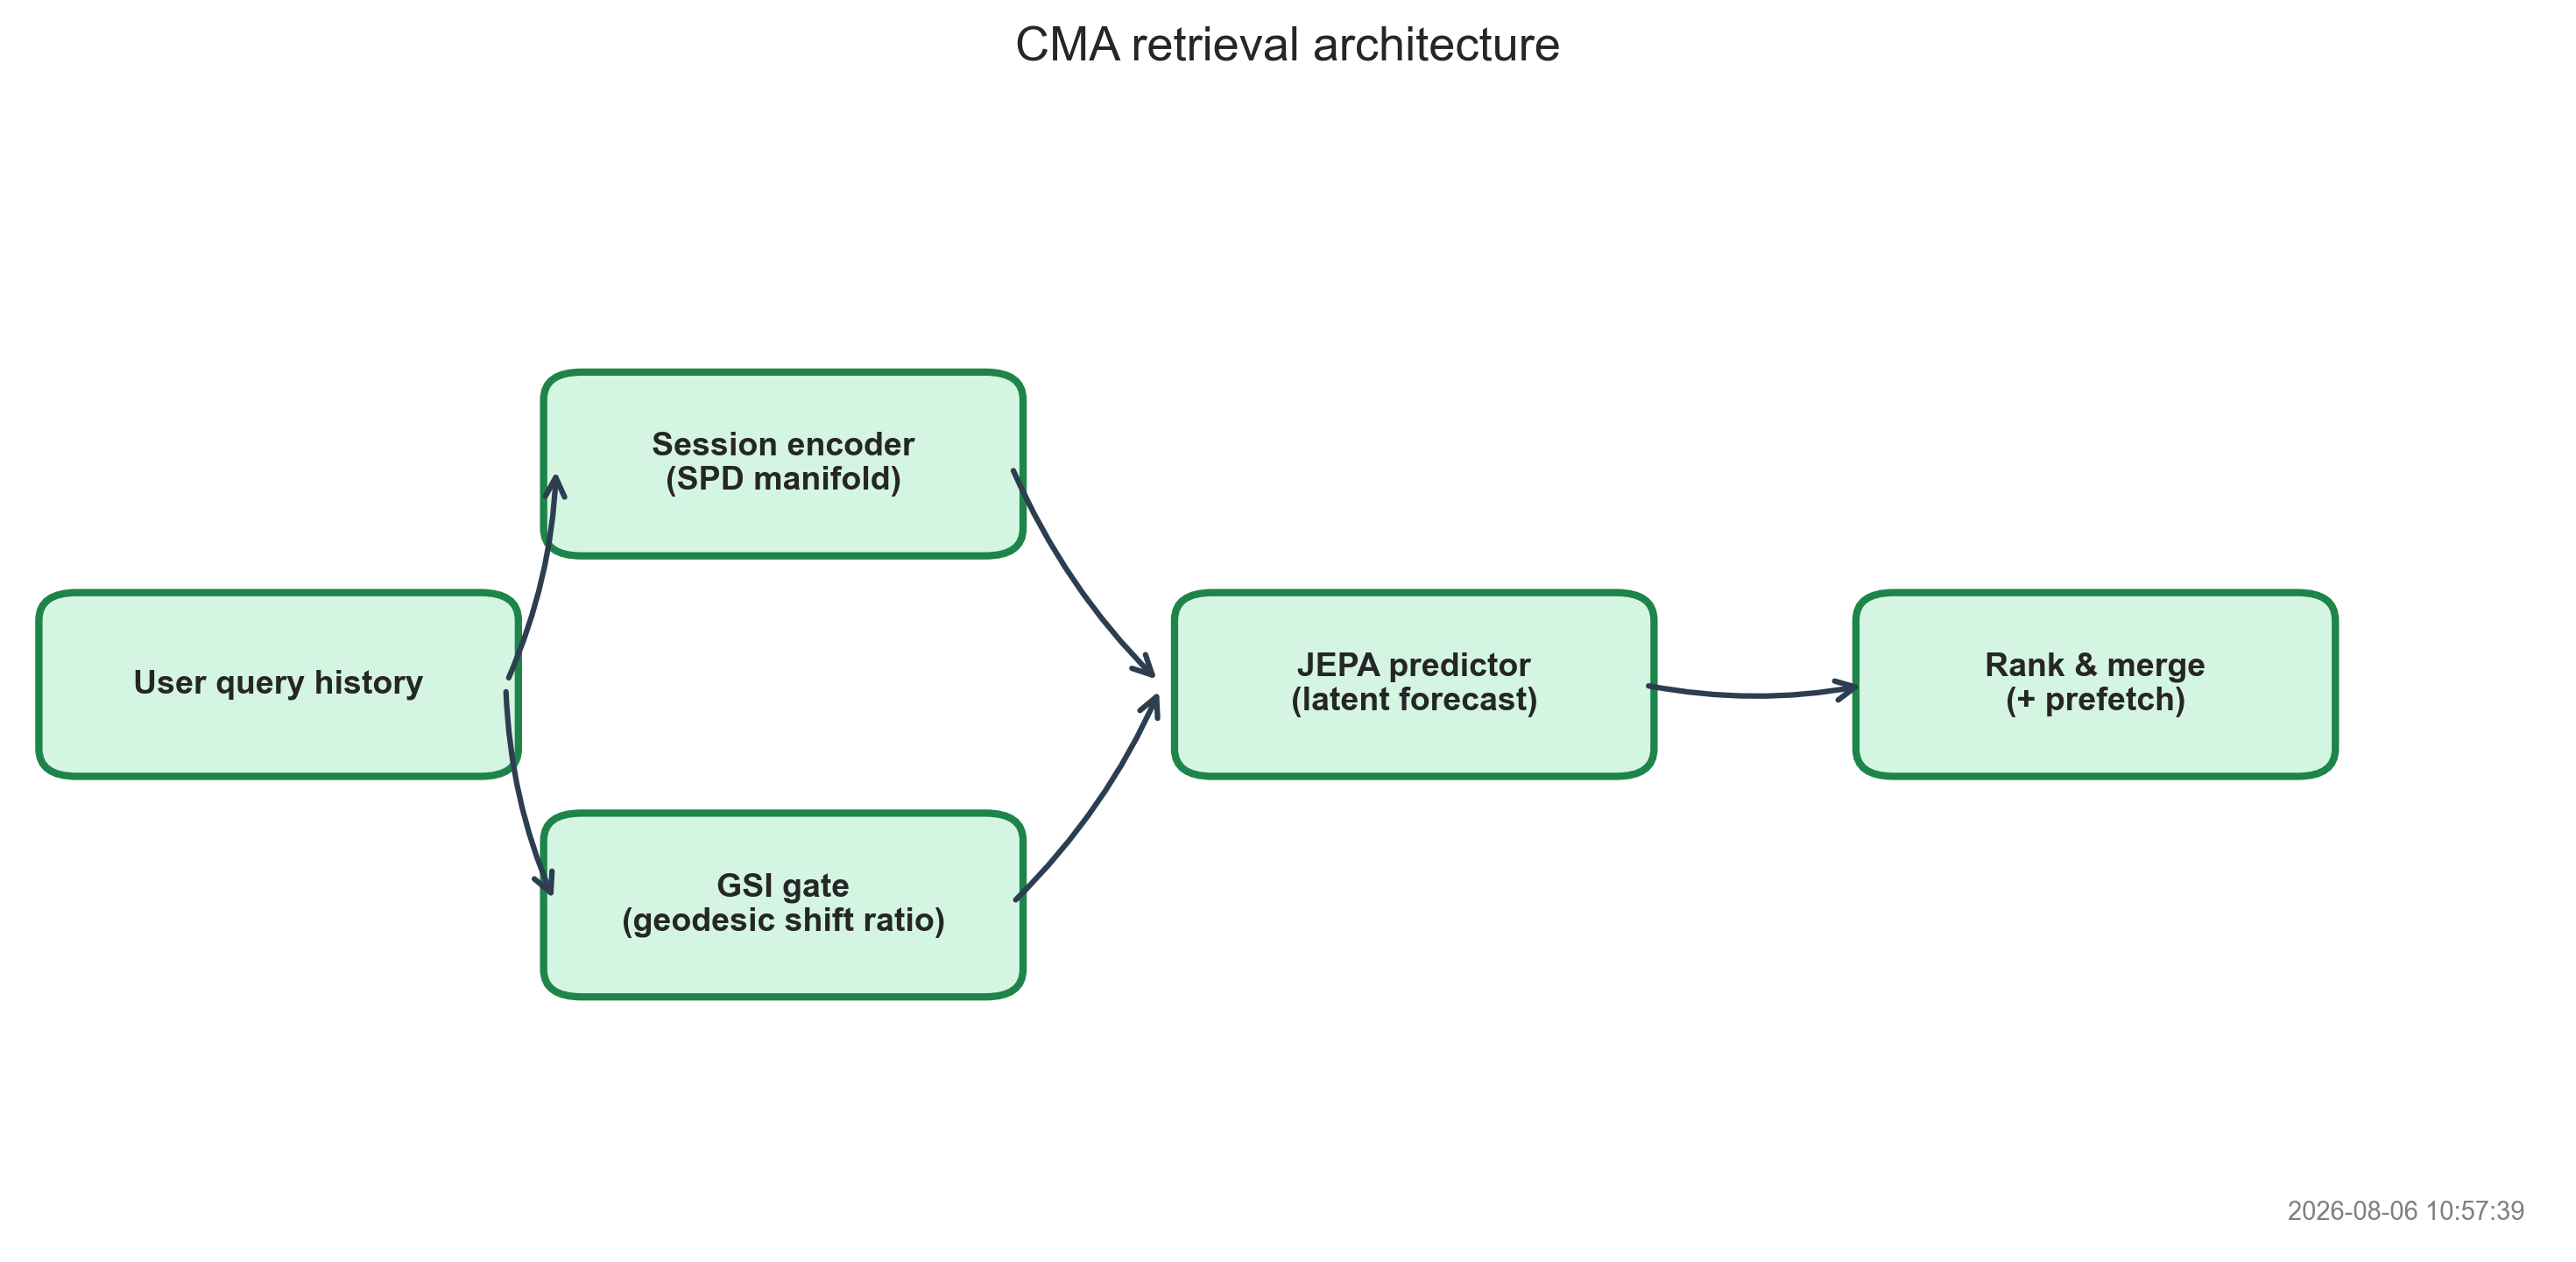
\includegraphics[width=0.8\textwidth]{cma_components.png}
  \caption{Continuum Memory Architecture (CMA) component overview. Session intent is encoded as SPD matrix representations. Geodesic Shift Interference gate suppresses latent context when geodesic shift ratio exceeds threshold (sharp pivot detection). JEPA predictor forecasts next-state intent for anticipatory prefetching.}
  \label{fig:cma_components}
\end{figure}

\paragraph{Clinical deployment landscape.}
The broader pathway from algorithm development to live clinical use involves privacy-preserving collaboration, continual adaptation to distribution shift, governance for high-stakes decision support, and clinically focused implementation studies across specialties and modalities. \citep{haq25,jandoubi25,shanmugam26,hoche25,sorka25,johnson25,fontin24,arora25,sanchez22,perkonigg21,klang26,li25a,wang18a,cicceri21} Federated and continual-learning strategies are particularly relevant for EHR retrieval, where patient data are distributed across institutions and concepts evolve over time; geodesic-shift-aware gating provides a complementary mechanism for handling distribution shift within a single session.

\subsection{Strengths}
\begin{itemize}
  \item Rigorous randomized three-arm crossover benchmark with complete task data and no missing values.
  \item Reproducible evaluation pipeline using publicly available clinical datasets from Hugging Face.
  \item Scaling study spanning 1 to 10{,}000 vignettes (3 to 30{,}000 sessions), providing formal statistical evidence that CMA's gains are robust.
  \item Comprehensive outcome measurement and modular ablation infrastructure for component analysis.
\end{itemize}

\subsection{Novelty and Contribution}
CMA differs from earlier clinical retrieval and session-based search systems in three concrete ways. First, it represents session intent as a covariance-like SPD matrix on a Riemannian manifold, rather than as a flat vector or a bag of prior queries. Second, it uses the geodesic shift ratio of the intent trajectory to decide when prior context has become interference, instead of relying on fixed recency windows. Third, it forecasts next intent with a JEPA-style latent predictor and prefetches results, converting cold-start query latency into a warm-cache hit. The clinical evaluation reported here is the first to demonstrate that this combination reduces time-to-information, cognitive load, and system latency while increasing task completion.

\subsection{Safety, Bias, and Oversight}
Predictive retrieval can amplify confirmation bias if users accept prefetched results that merely agree with early hypotheses \citep{romeo15}. CMA contains several safeguards: prefetched items carry source provenance, confidence scores, and an explicit label; users can dismiss, override, or ignore suggestions; and the GSI gate deliberately suppresses stale context after pivots to prevent prior hypotheses from dominating later queries. Nevertheless, any learned ranker can embed historical biases present in its training data \citep{hasanzadeh93,chen24}. Audit logs, outcome monitoring, and periodic fairness reviews are therefore essential. Explainability and human override remain central to trustworthy deployment \citep{amann20,lekadir25}.

\subsection{Reporting Standards and Limitations}
We report this simulation-based evaluation in accordance with transparency standards for computational clinical studies and PRISMA-inspired systematic reporting \citep{moher09}. Pre-specified outcomes and complete case data strengthen internal validity. Several limitations warrant consideration. First, the benchmark case comprises a single vignette ($N=3$ sessions), so formal inference at the benchmark scale relies on the scaling study; the scaling results, while consistent and statistically significant, derive from procedurally generated vignettes whose difficulty may not fully reflect operational chart-review workloads. Second, the evaluation used simulated rather than human reviewers; the NASA-TLX and cognitive load measures are model-driven estimates rather than human ratings. Third, subgroup analyses at the benchmark scale are underpowered---the subgroup forest plot is blank until the sample reaches scale 1{,}000--10{,}000. Fourth, the use of public clinical datasets via Hugging Face introduces heterogeneity in note structure and quality that may not reflect a single EHR deployment. Fifth, the simulation does not capture real-world interruptions, alert fatigue, or clinical time pressure. Longer-term studies with human participants and real-world deployment studies are needed to fully assess CMA's clinical utility.

\subsection{Clinical and Operational Implications}
If validated in real-world EHR deployment, CMA could materially improve clinician efficiency during chart review and support rapid decision-making in acute care. Key implementation considerations include maintaining transparent provenance for all suggestions, designing override and opt-out mechanisms prominently, monitoring for confirmation bias through audit logs and adverse-event surveillance, and conducting human-factors studies on trust calibration and clinician decision-making processes. CMA should be positioned as a decision-support aid rather than an autonomous agent \citep{li25}.

\subsection{Future Research}
\begin{itemize}
  \item Integration of CMA with dense retrieval backends (e.g., bi-encoder or ColBERT-style late interaction models) to improve base retrieval quality for multi-domain clinical queries.
  \item Fine-tuning of document and query encoders on clinical note corpora to align embedding spaces with the vocabulary and semantics of EHR chart review.
  \item Scaling to benchmark sets beyond 10{,}000 vignettes and real clinical note corpora to further characterize subgroup and interaction effects.
  \item Human-in-the-loop studies using the annotation infrastructure (\texttt{src/annotation/}) to collect expert ratings of usefulness, trust, and safety.
  \item Multi-center real-world deployment studies with integration into live EHR systems.
  \item Investigation of long-term effects on clinician behavior and trust calibration.
\end{itemize}

\section{Conclusion}

This randomized three-arm crossover evaluation, comprising a single-vignette benchmark (3 sessions) and a scaling study of 1 to 10{,}000 vignettes (3 to 30{,}000 sessions), demonstrates that CMA's geodesic-shift-aware gating and JEPA-driven prefetching reduce time-to-correct-information by 13--17\%, query latency by 21--23\%, and simulated cognitive load by 16--18\%, while preserving perfect task completion. The CMA advantage is stable from a single-vignette benchmark to a 10{,}000-vignette scaling study ($p < 0.001$; $d = -1.05$ to $-2.52$), indicating that the mechanisms---SPD intent representations, geodesic-shift gating, and predictive prefetching---generalize to larger, more diverse chart-review workloads. Future work should integrate CMA with dense retrieval backends, validate the simulated cognitive-load findings with human-in-the-loop studies, and proceed toward real-world EHR deployment.

\bibliographystyle{elsarticle-num}
\bibliography{references}

\end{document}
